\documentclass[compress]{beamer}
\usepackage{ifthen,verbatim}

\newcommand{\isnote}{}
\xdefinecolor{lightyellow}{rgb}{1.,1.,0.25}
\xdefinecolor{darkblue}{rgb}{0.1,0.1,0.7}

%% Uncomment this to get annotations
%% \def\notes{\addtocounter{page}{-1}
%%            \renewcommand{\isnote}{*}
%% 	   \beamertemplateshadingbackground{lightyellow}{white}
%%            \begin{frame}
%%            \frametitle{Notes for the previous page (page \insertpagenumber)}
%%            \itemize}
%% \def\endnotes{\enditemize
%% 	      \end{frame}
%%               \beamertemplateshadingbackground{white}{white}
%%               \renewcommand{\isnote}{}}

%% Uncomment this to not get annotations
\def\notes{\comment}
\def\endnotes{\endcomment}

\setbeamertemplate{navigation symbols}{}
\setbeamertemplate{headline}{\mbox{ } \hfill
\begin{minipage}{5.5 cm}
\vspace{-0.75 cm} \small
\end{minipage} \hfill
\begin{minipage}{4.5 cm}
\vspace{-0.75 cm} \small
\begin{flushright}
\ifthenelse{\equal{\insertpagenumber}{1}}{}{Jim Pivarski \hspace{0.2 cm} \insertpagenumber\isnote/\pageref{numpages}}
\end{flushright}
\end{minipage}\mbox{\hspace{0.2 cm}}\includegraphics[height=1 cm]{../cmslogo} \hspace{0.1 cm} \includegraphics[height=1 cm]{../tamulogo} \hspace{0.01 cm} \vspace{-1.05 cm}}

\newcommand{\s}[1]{{\mbox{\scriptsize #1}}}

\begin{document}
\begin{frame}
\vfill
\begin{center}
\textcolor{darkblue}{\Large Updated Internal Alignment of CSC Rings}

\vfill
\begin{columns}
\column{0.3\linewidth}
\begin{center}
\large
Jim Pivarski
\end{center}
\end{columns}

\begin{columns}
\column{0.3\linewidth}
\begin{center}
\scriptsize
{\it Texas A\&M University}
\end{center}
\end{columns}

\vfill
 8 November, 2010

\end{center}
\end{frame}

%% \begin{notes}
%% \item This is the annotated version of my talk.
%% \item If you want the version that I am presenting, download the one
%% labeled ``slides'' on Indico (or just ignore these yellow pages).
%% \item The annotated version is provided for extra detail and a written
%% record of comments that I intend to make orally.
%% \item Yellow notes refer to the content on the {\it previous} page.
%% \item All other slides are identical for the two versions.
%% \end{notes}

\small

\begin{frame}
\frametitle{New alignment motivation}
\begin{itemize}
\item Previous internal ring alignments with beam-halo data:
\begin{itemize}
\item \textcolor{darkblue}{Sep.\ 2008} ``first beam'' (9 minutes) with $\vec{B}=0$, only two rings (ME$-$2/1, $-$3/1), not uploaded to the database
\item \textcolor{darkblue}{Dec.\ 2009} ``first collisions'' (21 days) with $\vec{B}=3.8$~T, too few halo events
\item \textcolor{darkblue}{Mar.\ 2010} ``Tertiary Collimator Triplet (TCT) test'' (40~minutes) with $\vec{B}=3.8$~T, new technique to use photogrammetry to supplement missing overlaps, aligned all chambers: \textcolor{darkblue}{current CSC geometry}
\end{itemize}
\item \textcolor{darkblue}{Jun.--Sep.\ 2010} beam-halo during collisions (83 days):
\begin{itemize}
\item 10$\times$ more events than the TCT dataset
\item collisions muons allow us to pre-align $\phi_y$ (potentially reduces a systematic error)
\item proposed new internal alignment (to be combined with whole-ring alignments)
\end{itemize}
\end{itemize}
\end{frame}

\begin{frame}
\frametitle{Reminder of the method}
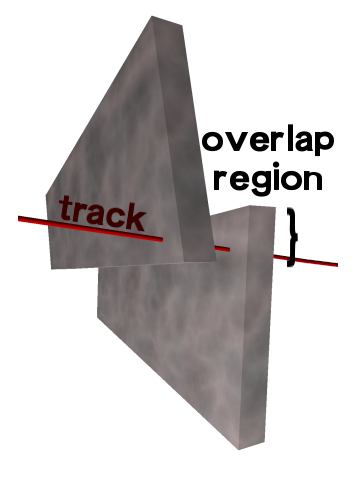
\includegraphics[height=3.2 cm]{overlaps.png}\hfill
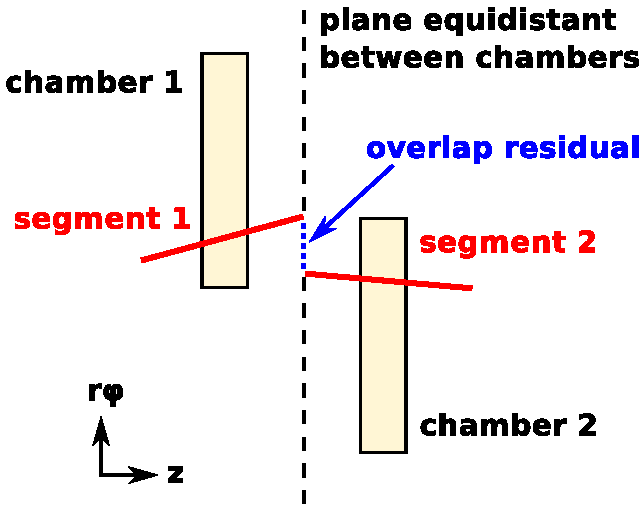
\includegraphics[height=3.2 cm]{overlaps_diagram.pdf}\hfill
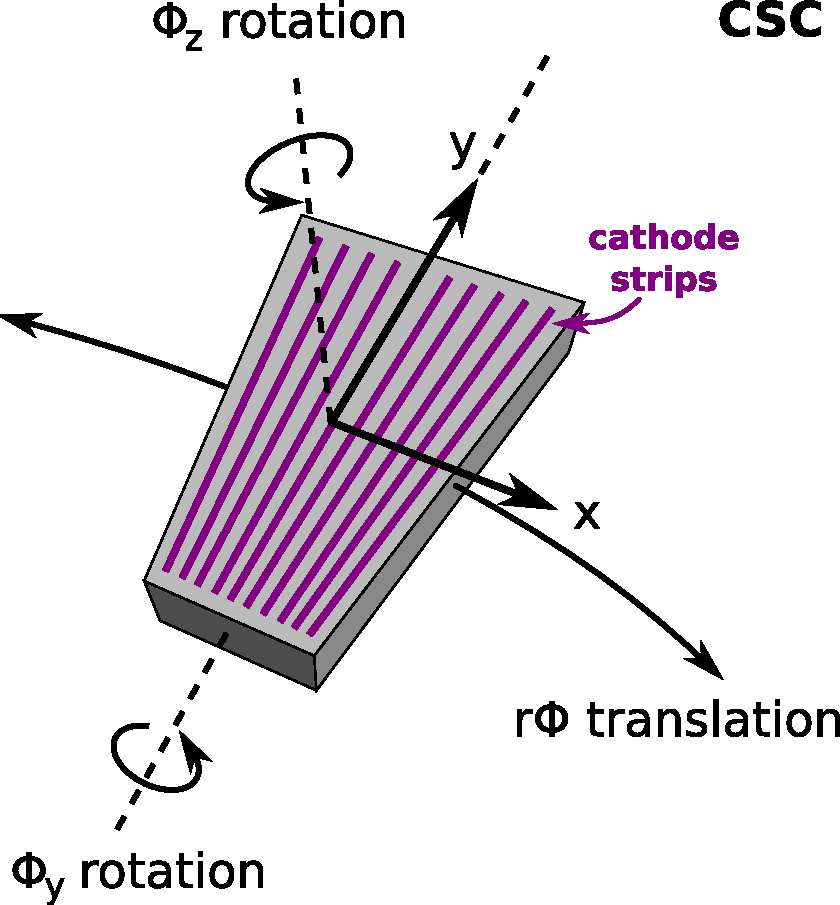
\includegraphics[height=3.2 cm]{csc_coordinates.pdf}

\begin{enumerate}
\item Align $\phi_y$ angles from collisions (next slide)
\item Select beam-halo tracks that cross overlap of neighboring CSCs
\item Quantify relative misalignment of the two chambers with overlap residual (above)
\item Solve for best fit of all relative measurements:
\[\chi^2 = \sum_{m_{ij}}^\s{constraints} \frac{(m_{ij} - A_i +
  A_j)^2}{{\sigma_{ij}}^2} + \mbox{ Lagrange multiplier} \]

where $m_{ij} \pm \sigma_{ij}$ is a measurement between $i$ and $j$
and $A_i$, $A_j$ are alignment corrections (variables to minimize
$\chi^2$) in $r\phi$ and $\phi_z$
\end{enumerate}
\end{frame}

\begin{frame}
\frametitle{$\phi_y$ pre-alignment}

\begin{columns}
\column{0.4\linewidth}
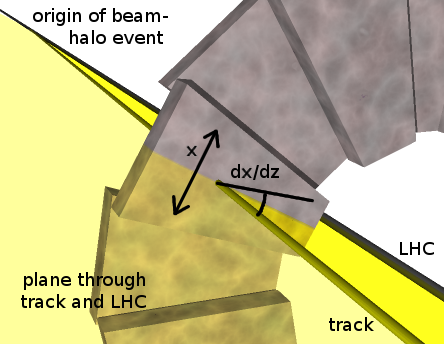
\includegraphics[width=\linewidth]{track_lhc_plane_closeup.png}

\column{0.6\linewidth}
\begin{itemize}
\item $\phi_y$ not measured by photogrammetry
\item First $\phi_y$ alignment attempt with 2008 $\vec{B}=0$ data by
  assuming that beam-halo points back to a long, straight LHC beamline
  (not used)
\item Attempted to align $\phi_y$ with beam-halo overlaps method, but
  resolution is poor (fixed to zero in Mar.~2010 alignment)
\end{itemize}
\end{columns}

\hfill 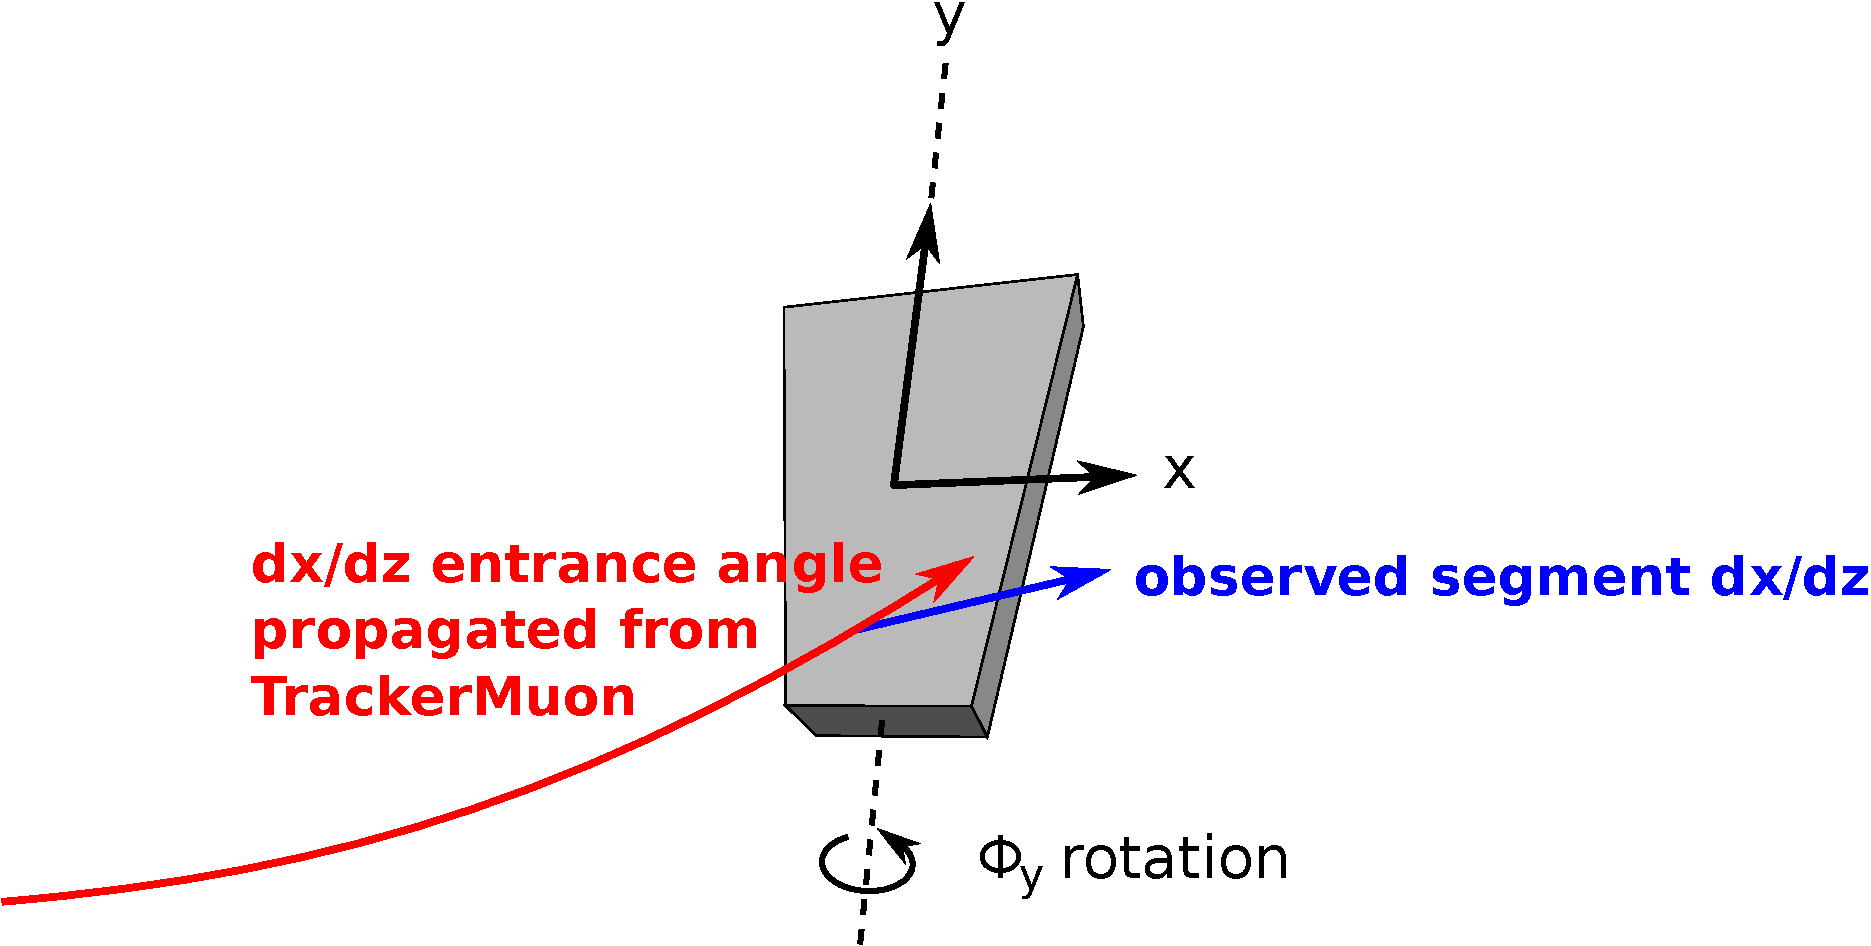
\includegraphics[width=0.8\linewidth]{collisions_phiy.pdf}

\vspace{-4.3 cm}
\begin{itemize}
\item New measurement with \\ collisions is now possible

(used 2.9~pb$^{-1}$)
\end{itemize}

\vspace{4 cm}
\end{frame}

\begin{frame}
\frametitle{$\phi_y$ pre-alignment}

\textcolor{darkblue}{Comparison of 3 (4?) methods over the years:} \hfill (now using collisions)

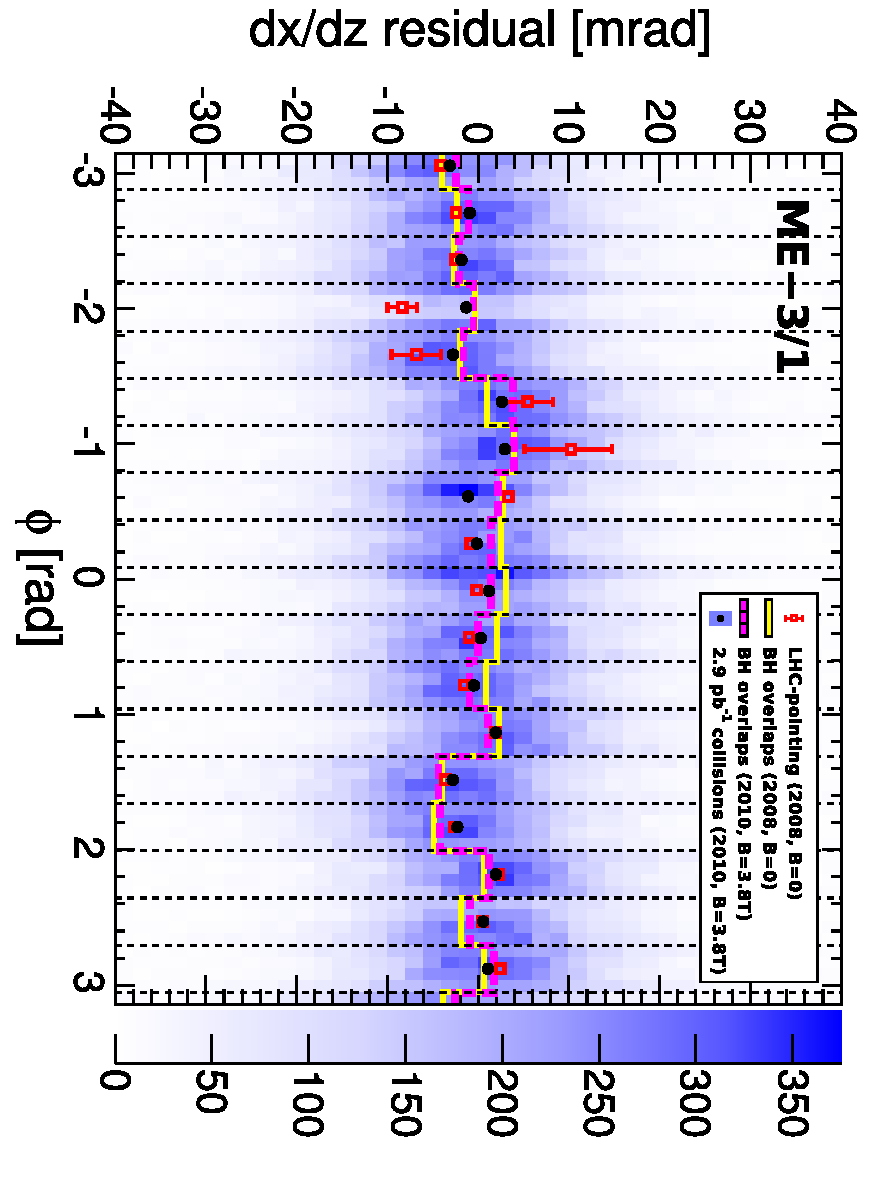
\includegraphics[height=0.9\linewidth, angle=90]{mem3phiy_all.pdf}
\end{frame}

\begin{frame}
\frametitle{Beam-halo data quality}

\begin{itemize}
\item Occupancy maps of the overlap regions (bottom: suppressed scale)
\item 7 problems were fixed (all in ME1/1); 1 new problem \mbox{(ME$-$1/2/4-5)\hspace{-1 cm}}
\end{itemize}

\begin{columns}
\column{0.5\linewidth}
\centering Mar.~2010 (TCT)

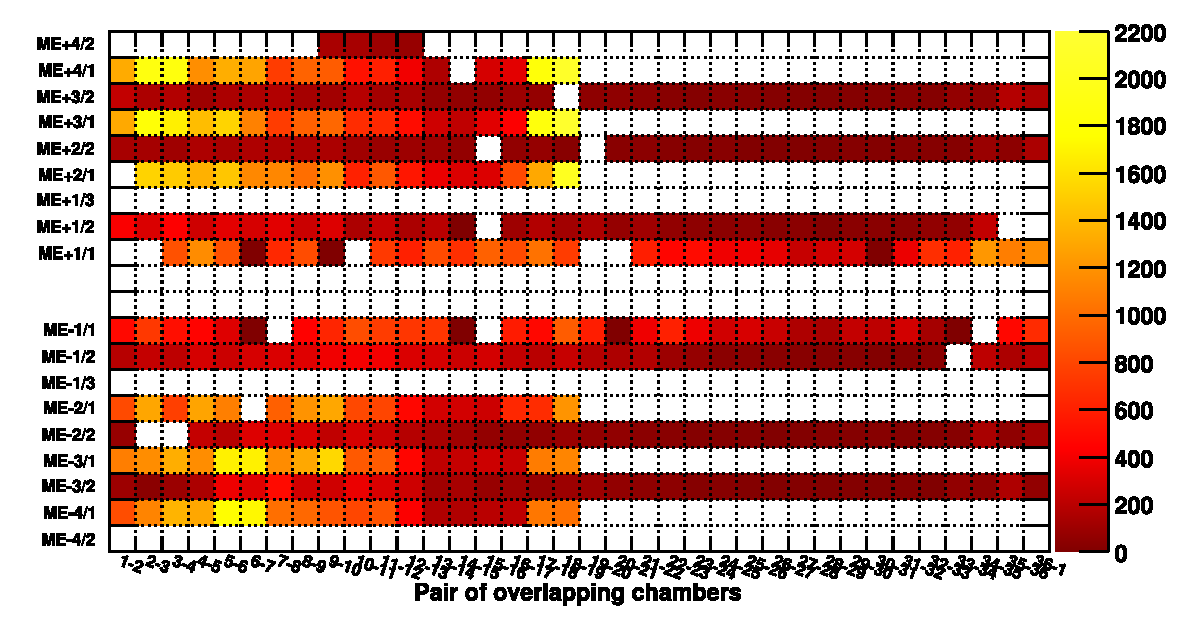
\includegraphics[width=\linewidth]{occupancy_March2010.pdf}

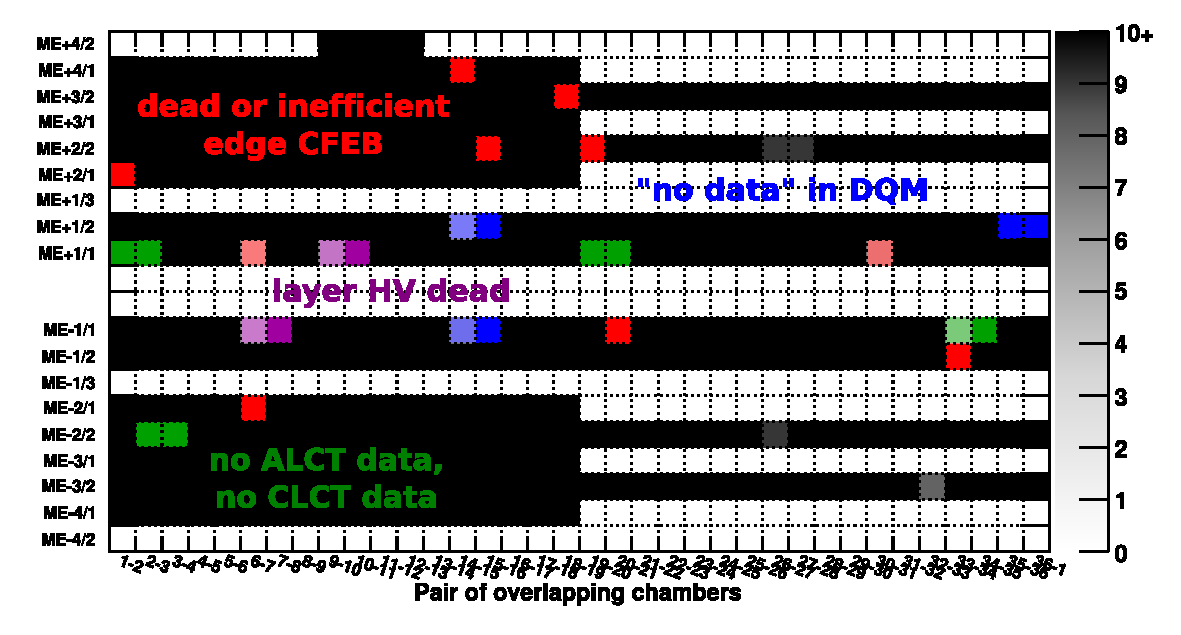
\includegraphics[width=\linewidth]{occupancy_problems_March2010.pdf}

\column{0.5\linewidth}
\centering Summer~2010 (collisions)

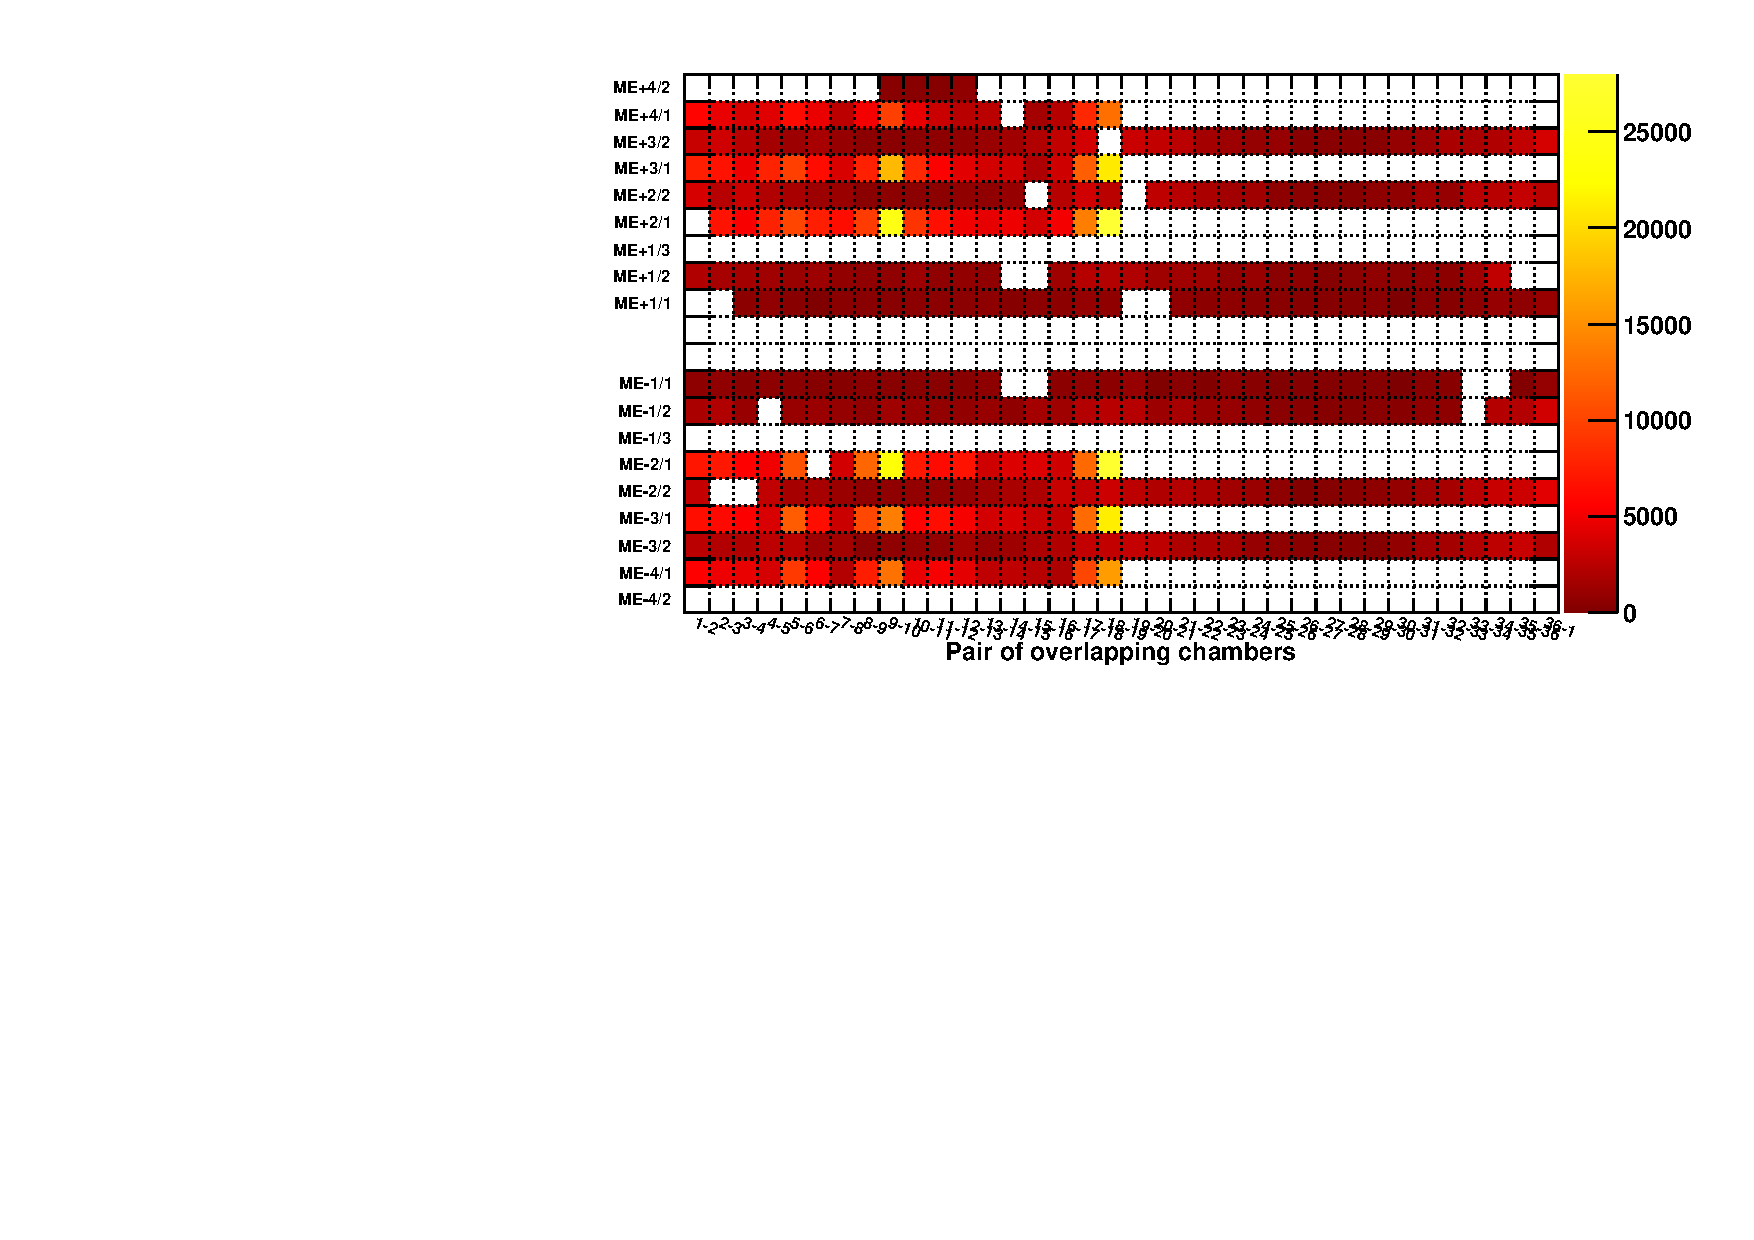
\includegraphics[width=\linewidth]{occupancy_Oct2010.pdf}

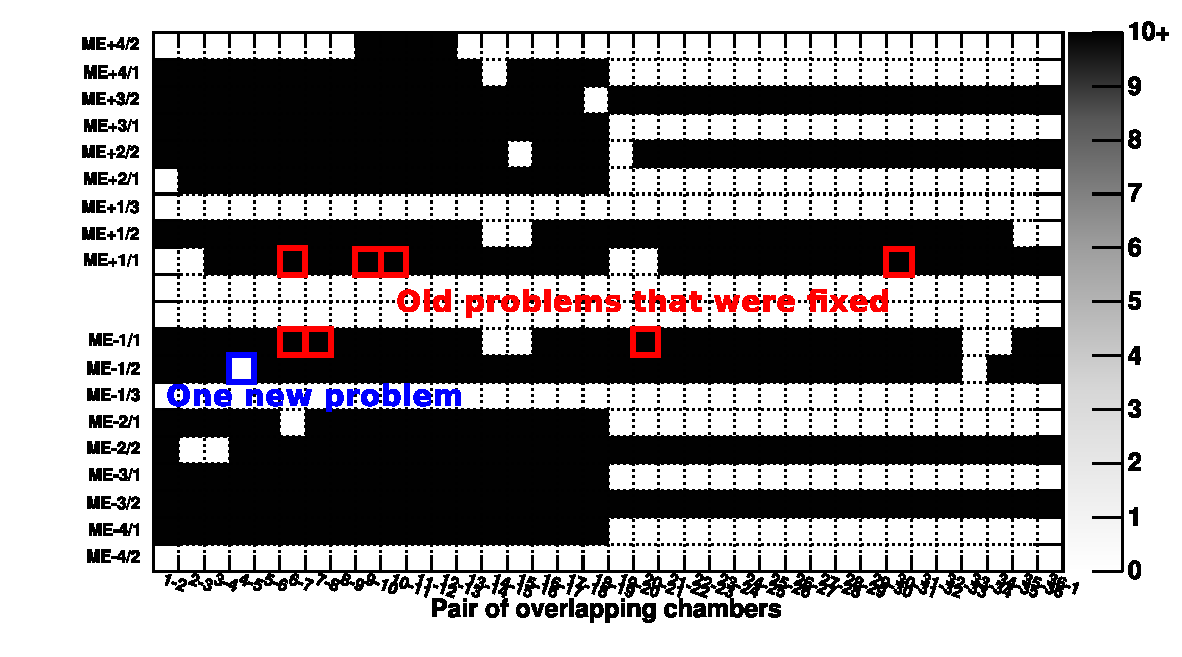
\includegraphics[width=\linewidth]{occupancy_problems_Oct2010.pdf}

\end{columns}
\end{frame}

\begin{frame}
\frametitle{Beam-halo data quality}

\begin{itemize}
\item Momentum cut ($|\vec{p}|$ measured primarily by {\it radial} magnetic field)

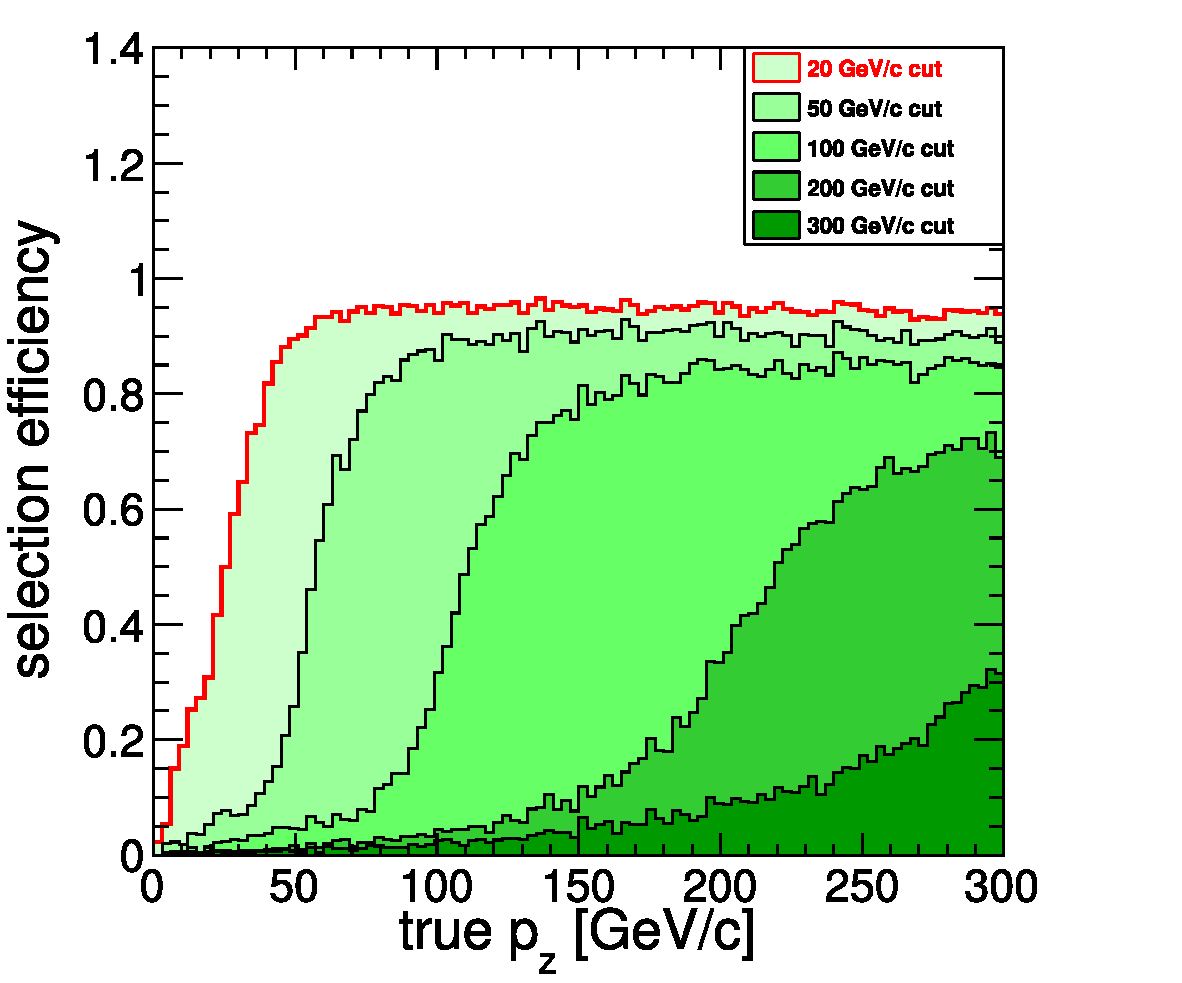
\includegraphics[height=3.5 cm]{trackfit_turnon.pdf}
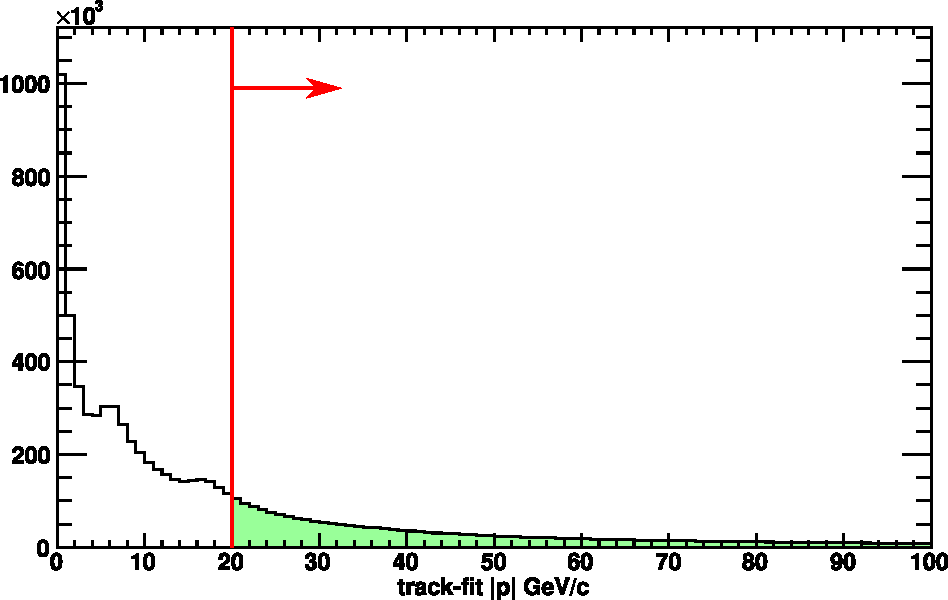
\includegraphics[height=3.5 cm]{momentum_Oct2010.pdf}

\item Radial entrance angle $dr/dz$ (horizontalness)

\mbox{\hspace{-1.3 cm}
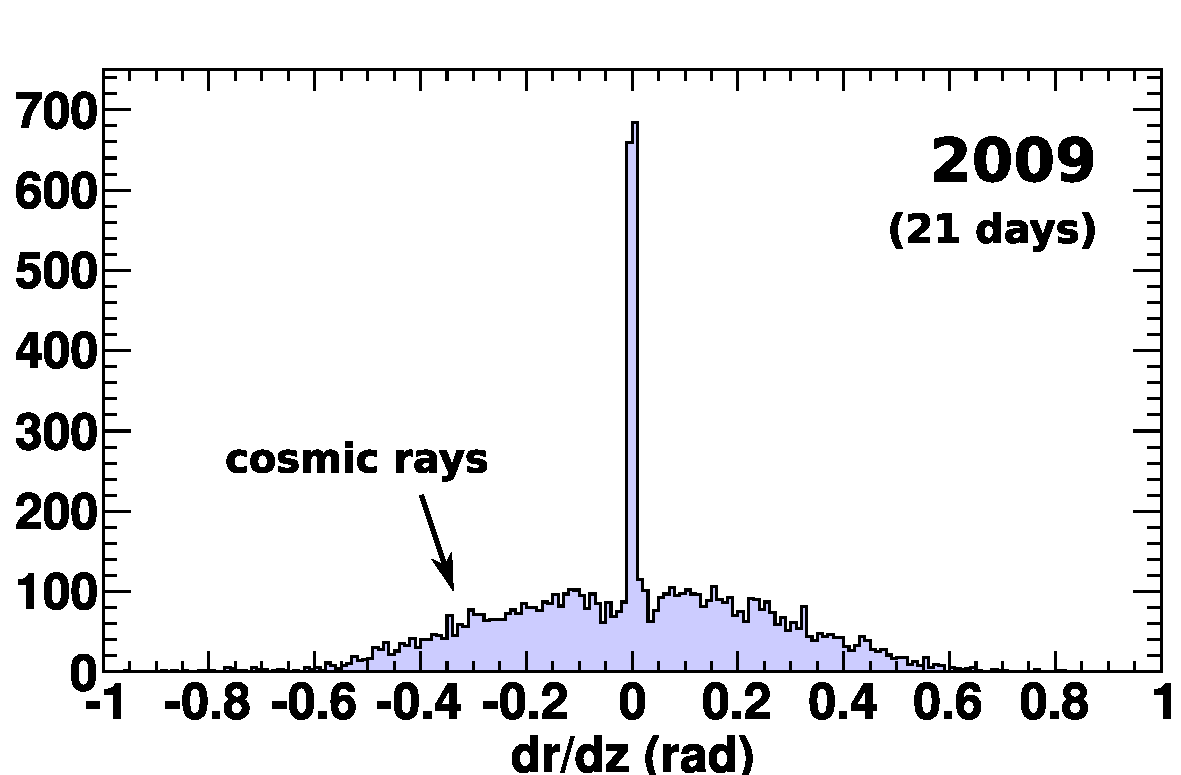
\includegraphics[height=2.6 cm]{drdz_Dec2009.pdf}
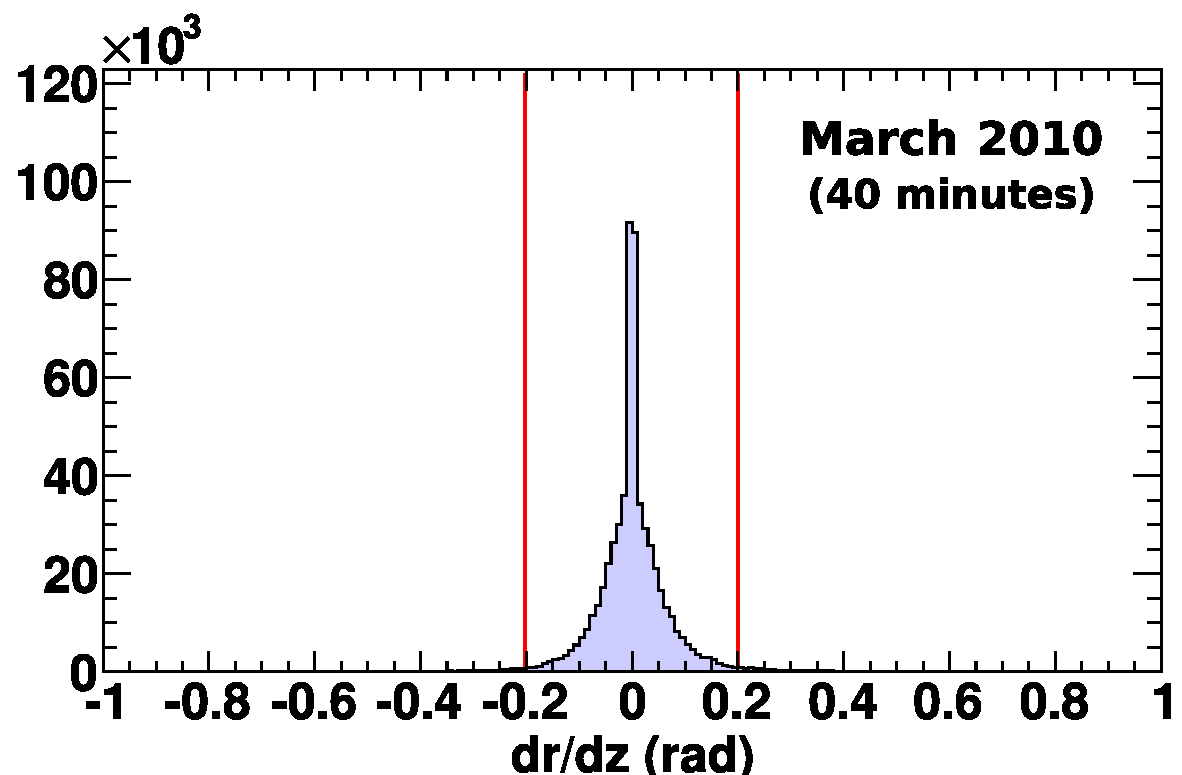
\includegraphics[height=2.6 cm]{drdz_March2010.pdf}
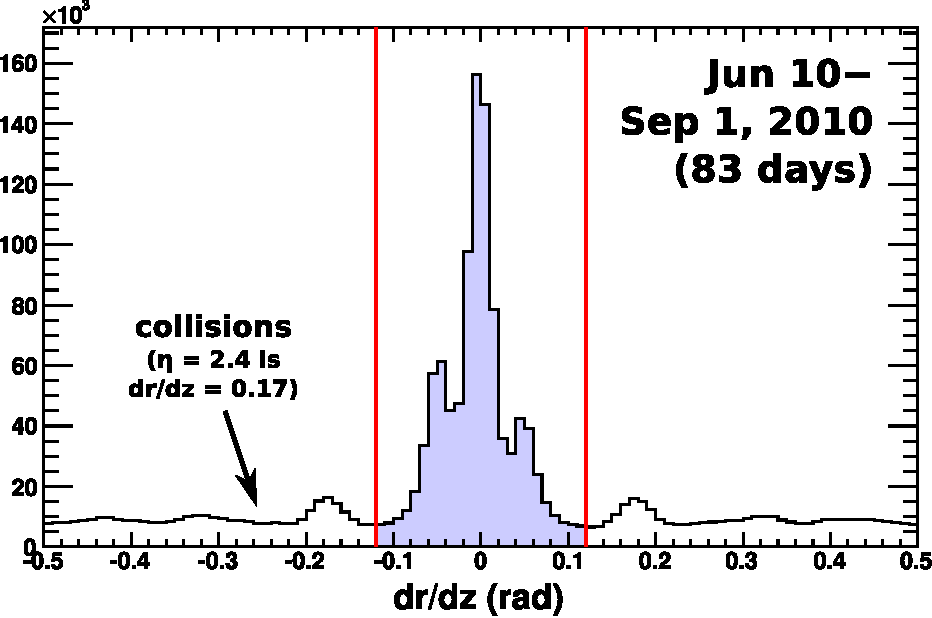
\includegraphics[height=2.6 cm]{drdz_Oct2010.pdf}}

\end{itemize}
\end{frame}

\begin{frame}
\frametitle{Residuals}
\begin{itemize}
\item The short track-segments used in overlaps alignment are not very
  sensitive to the size of the $\phi_y$ corrections (nor are the
  final results)

\begin{center}
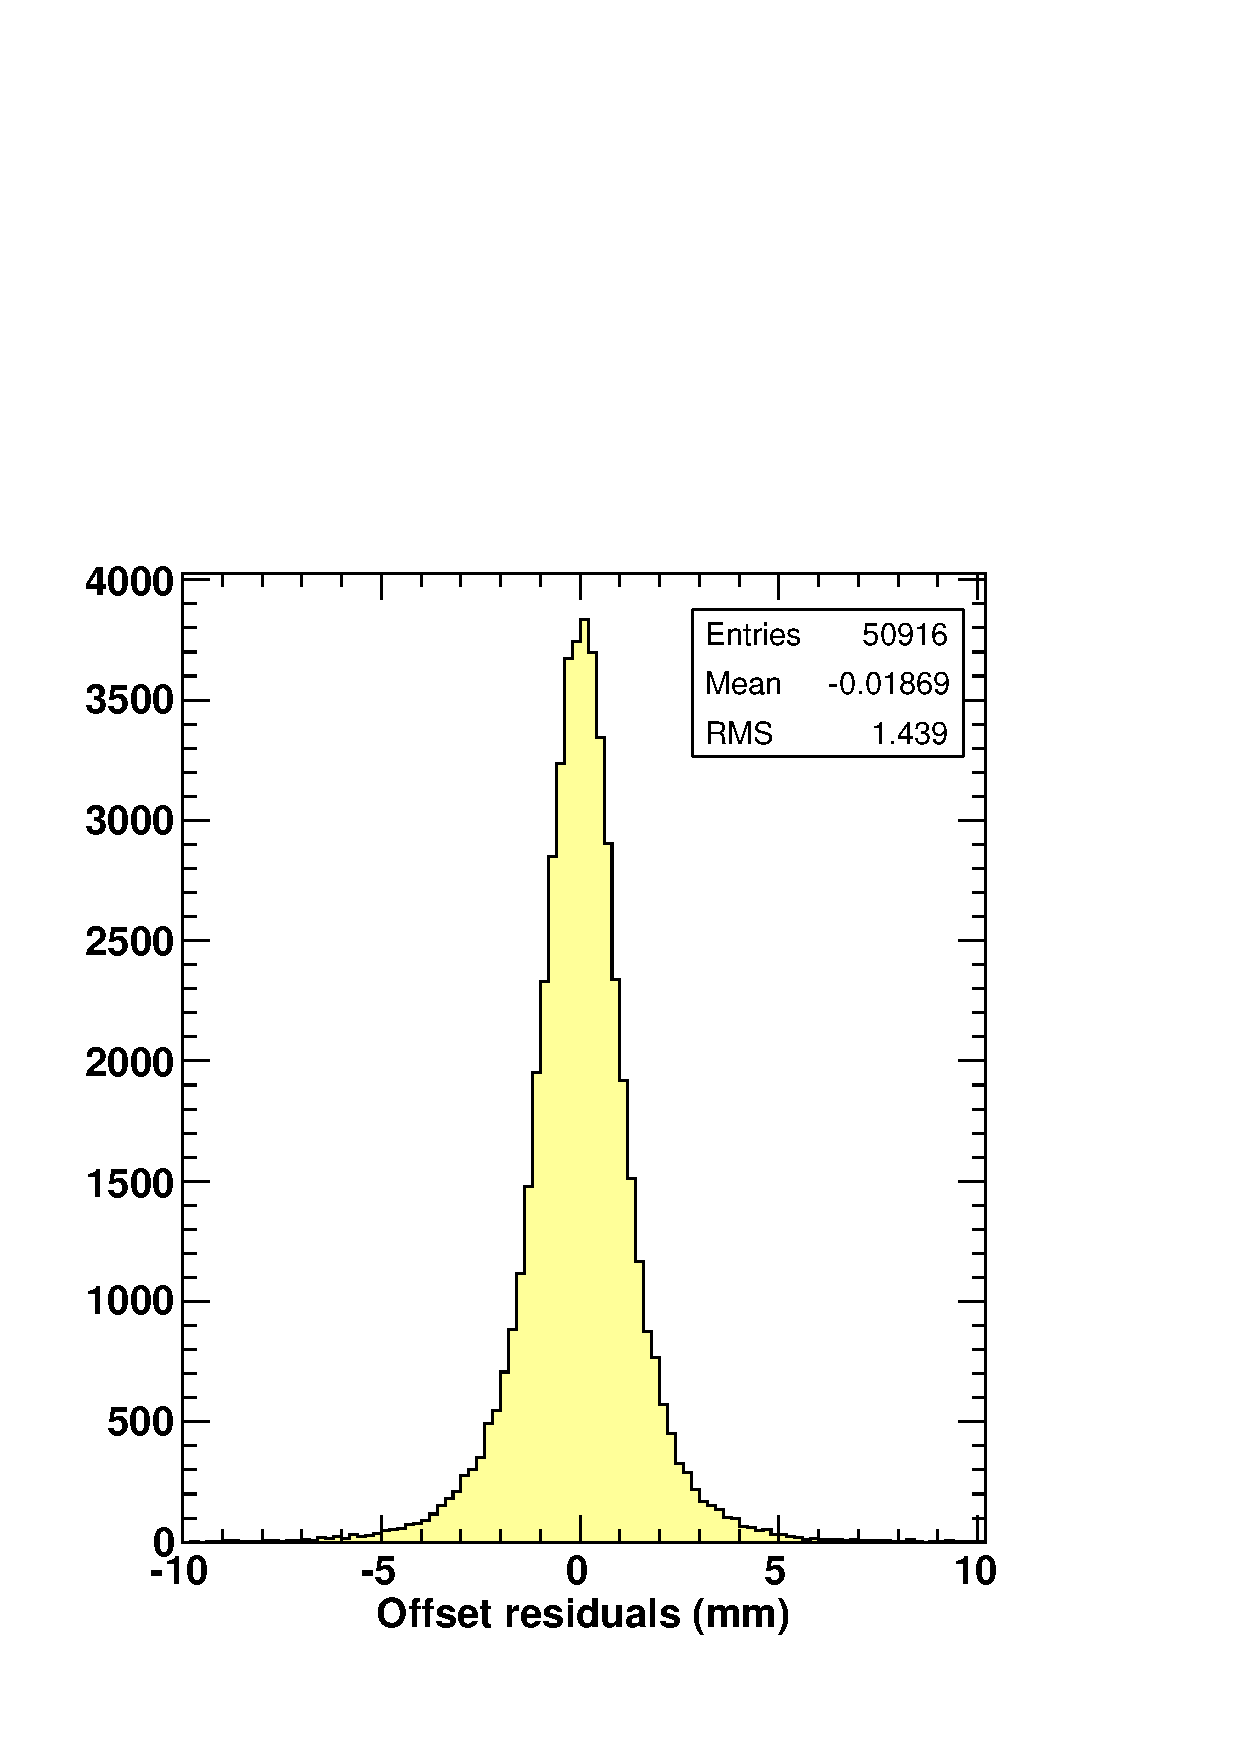
\includegraphics[width=0.5\linewidth]{offsetResiduals_badphiy.pdf}
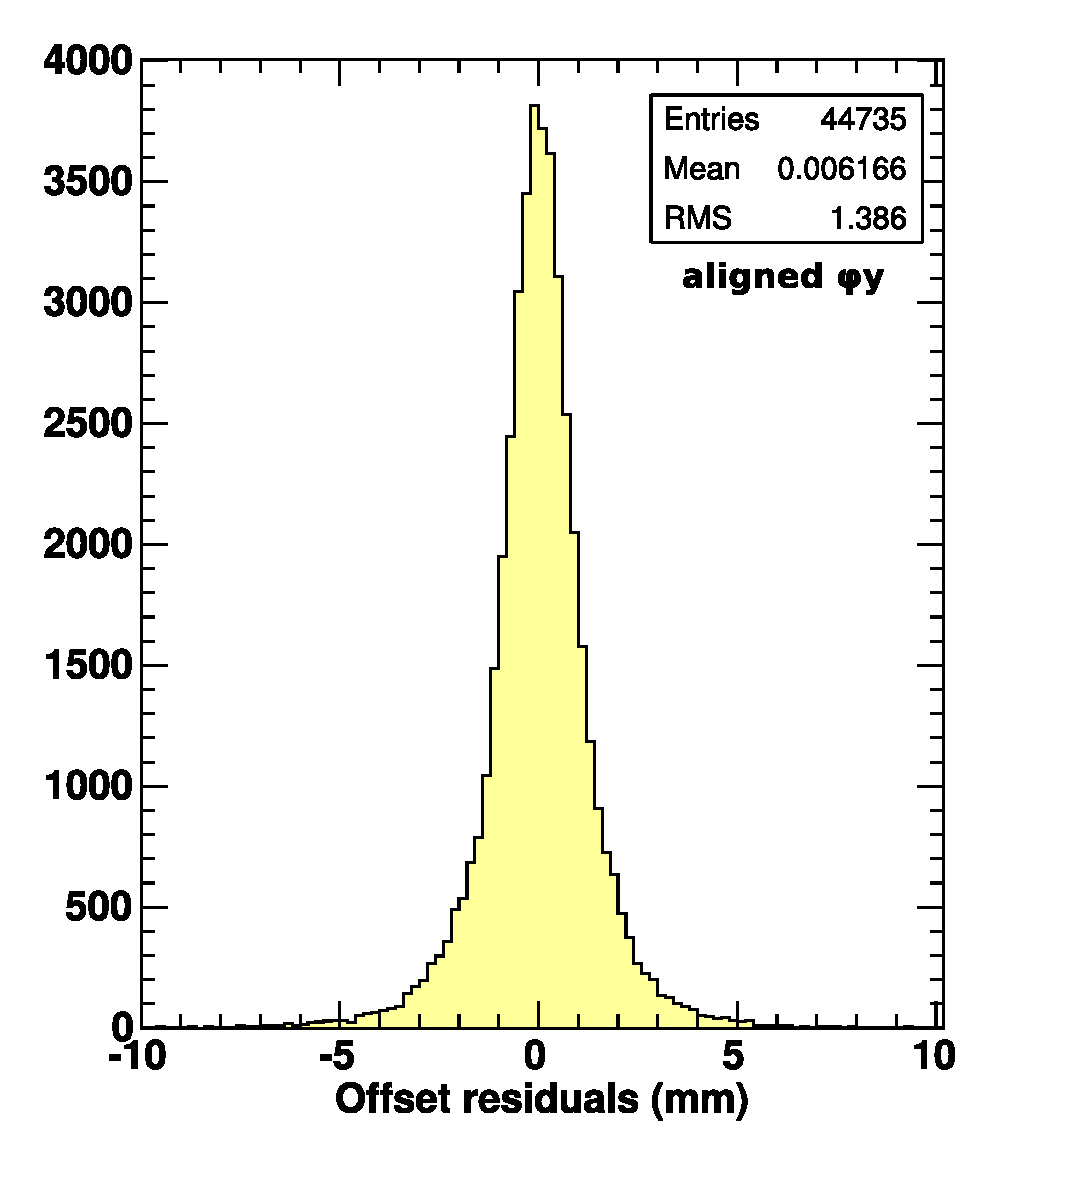
\includegraphics[width=0.5\linewidth]{offsetResiduals_goodphiy.pdf}
\end{center}
\end{itemize}
\end{frame}

\begin{frame}
\frametitle{Results: March $\to$ summer}

\begin{itemize}
\item Differences in $r\phi$ chamber positions between March and summer:

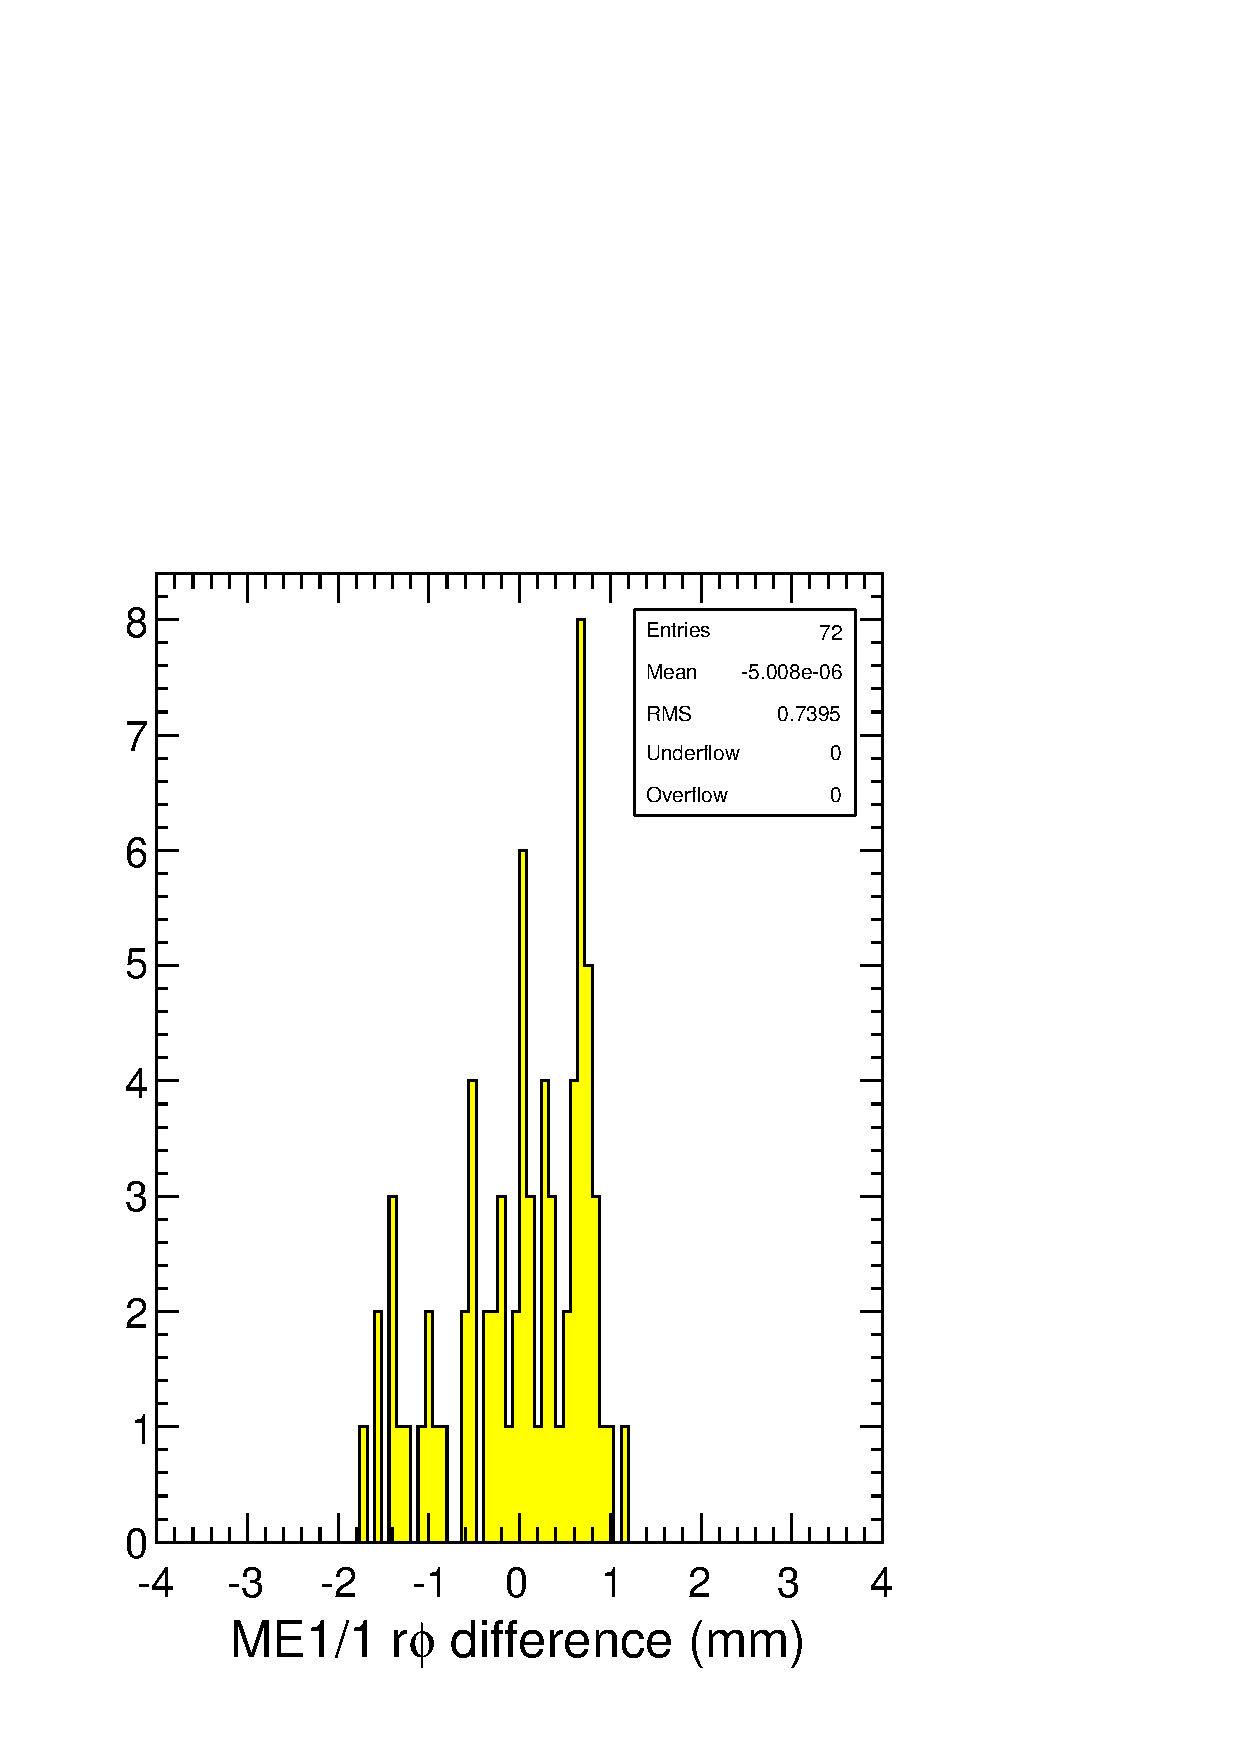
\includegraphics[width=0.32\linewidth]{TCTtoCollisions_me11.pdf}
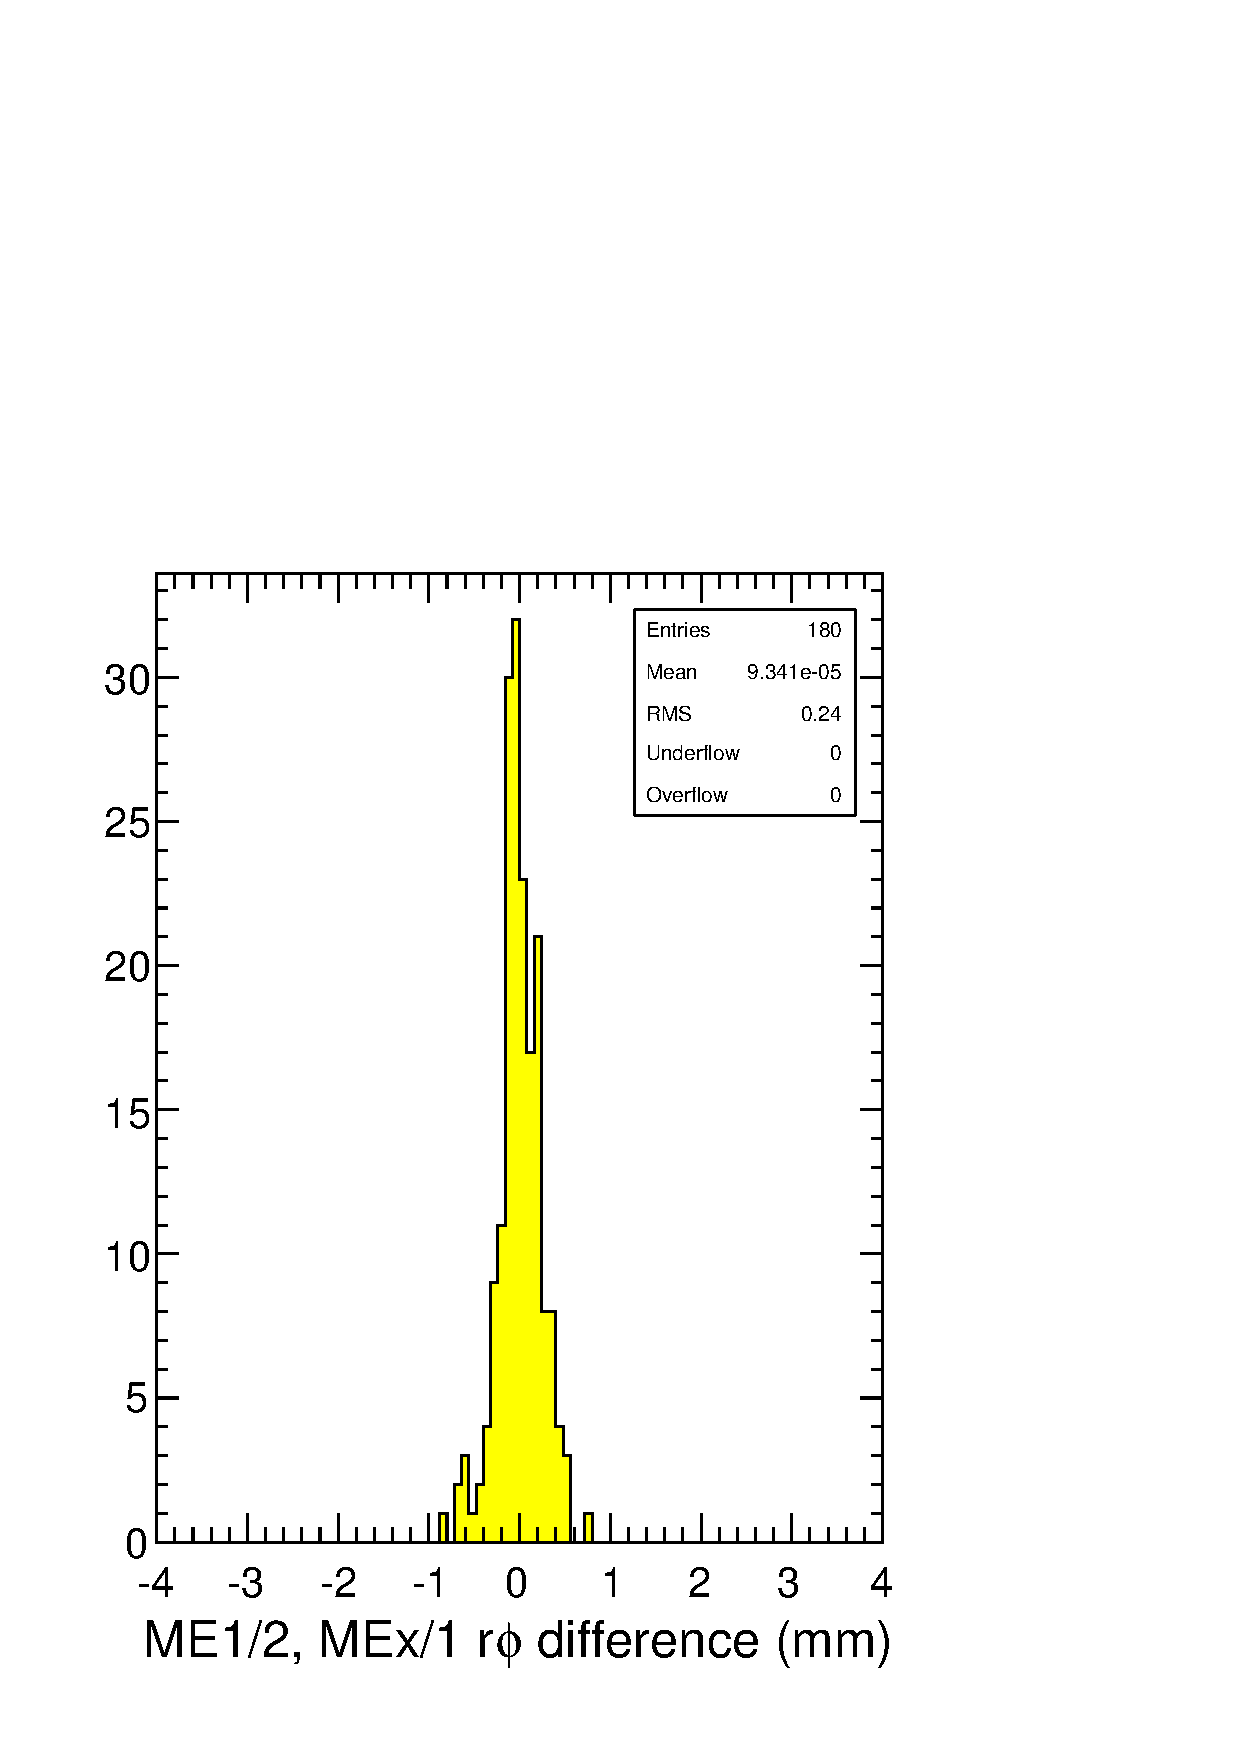
\includegraphics[width=0.32\linewidth]{TCTtoCollisions_inner.pdf}
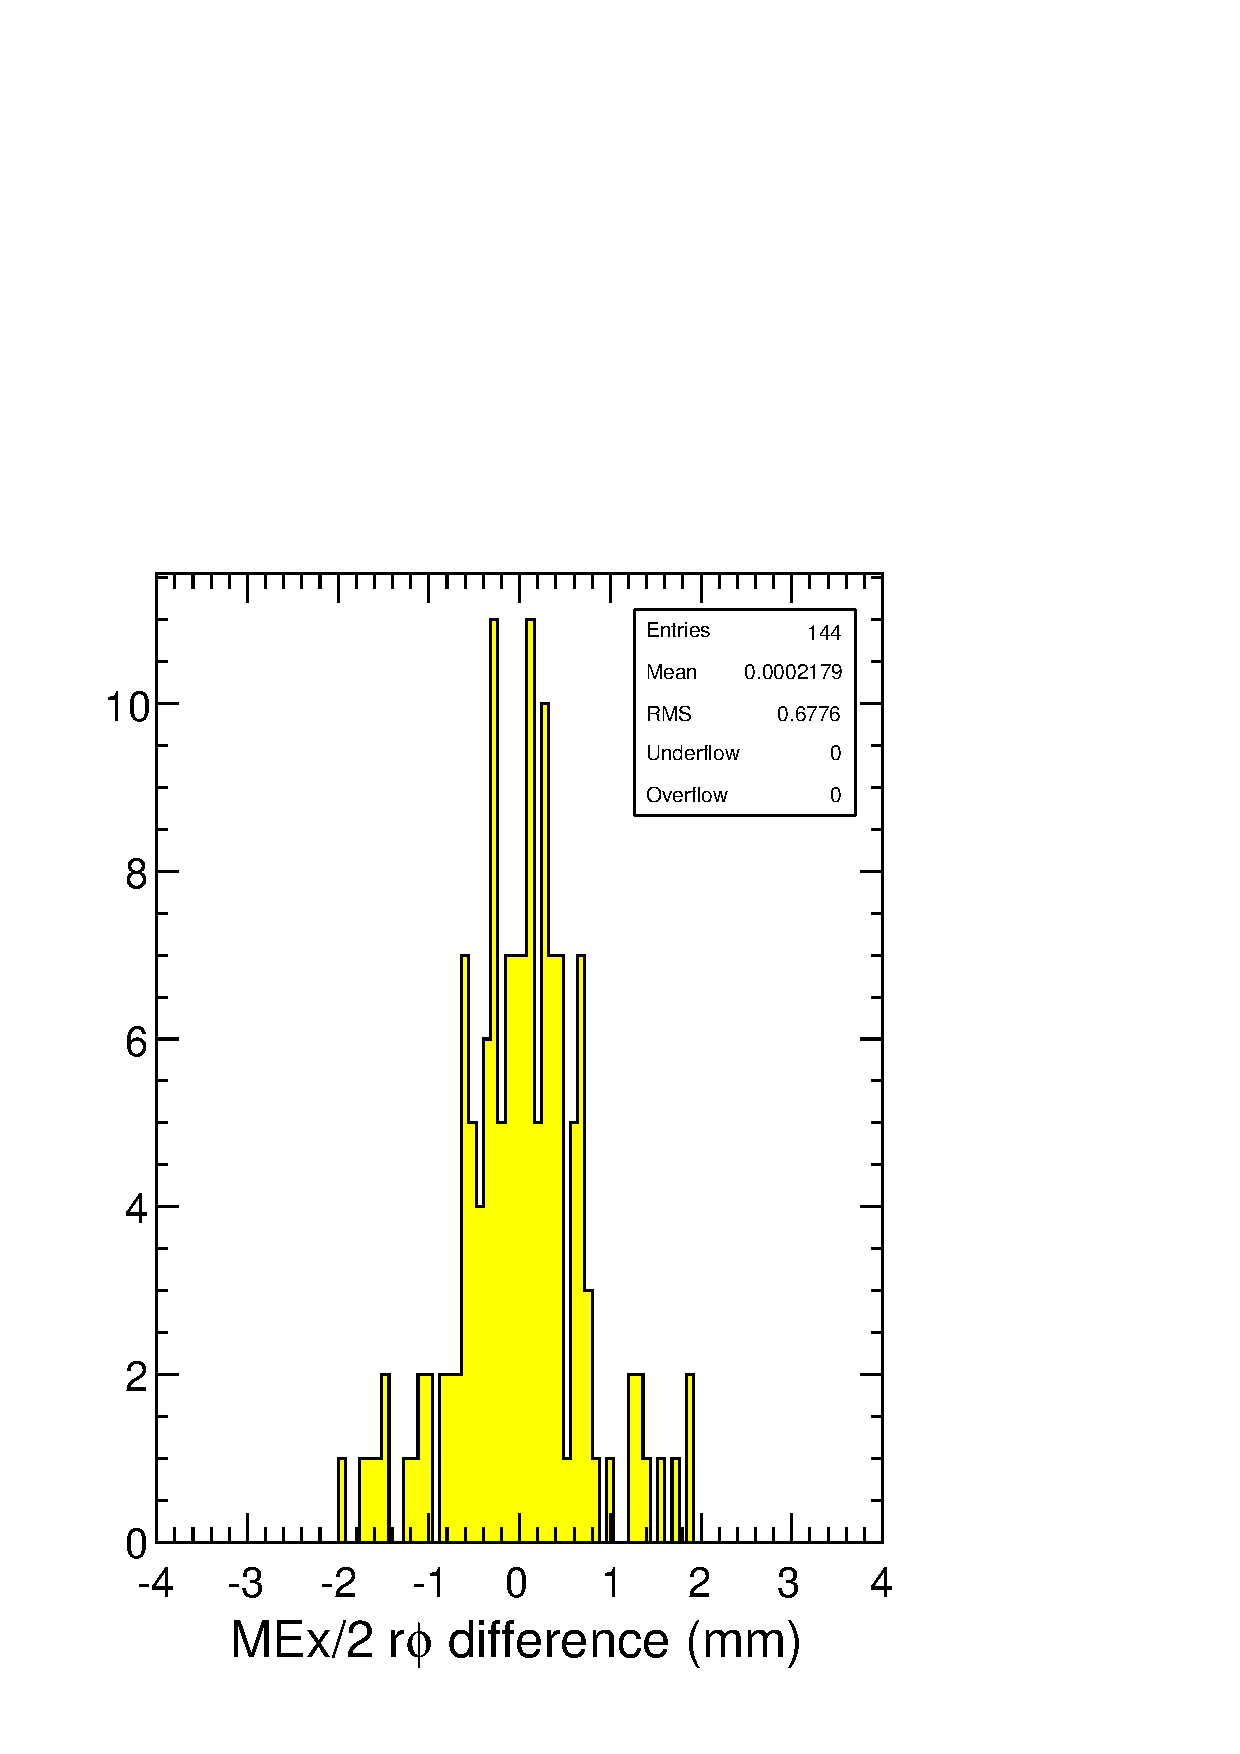
\includegraphics[width=0.32\linewidth]{TCTtoCollisions_outer.pdf}

\item ME1/1 benefited from the corrected chambers (next page)
\item ME1/2, $x$/1 (where $x \ge 2$) are closest to the beam: always
  get high beam-halo statistics
\item ME$x$/2 benefited the most from the $10\times$ increase in statistics
\end{itemize}
\end{frame}

\begin{frame}
\frametitle{Results: March $\to$ summer}

\begin{itemize}
\item Biggest ME1/1 March $\to$ summer differences in the interfaces between ME$+$1/1/6-7 and 30-31
\item These are two of the missing-data overlaps in March that have since been repaired:

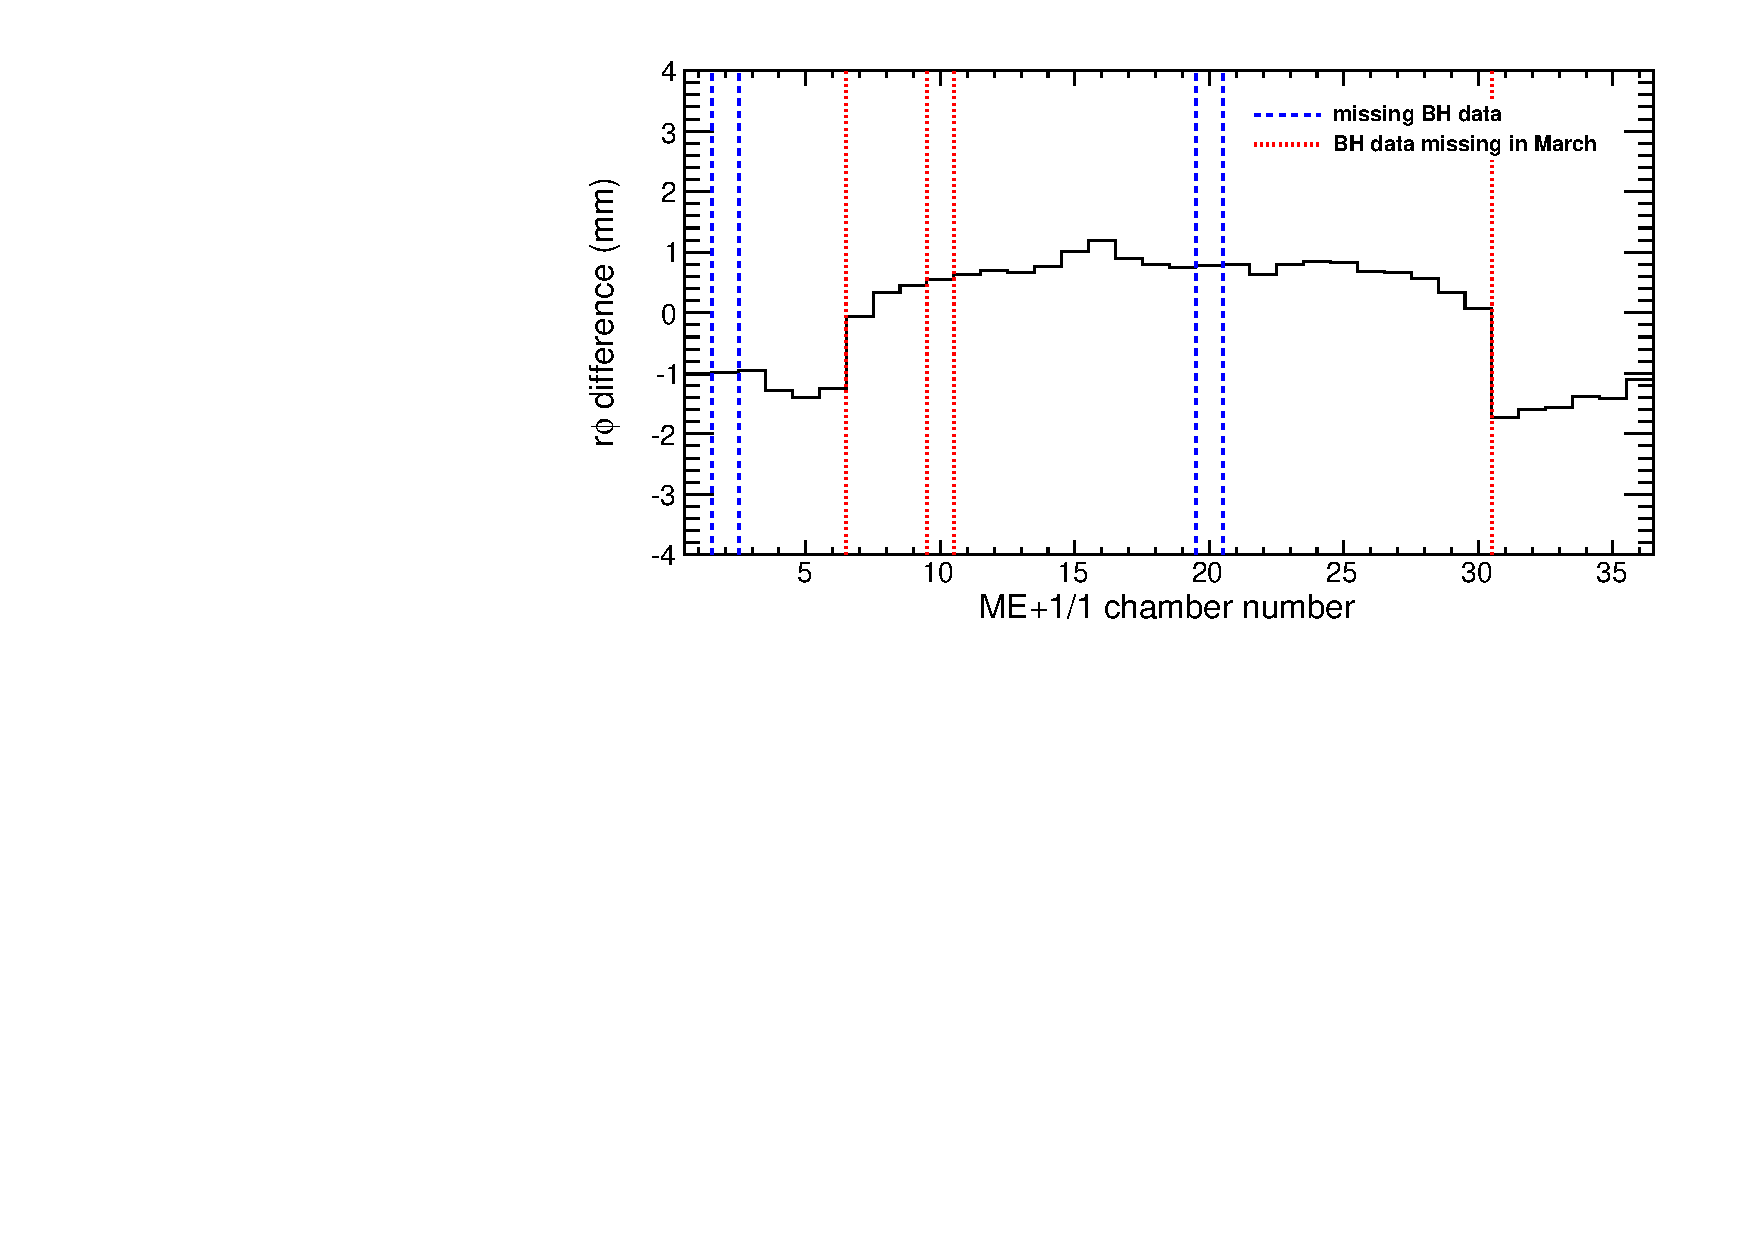
\includegraphics[width=\linewidth]{TCTtoCollisions_mep11.pdf}

\item Technique of constraining missing information with
  photogrammetry doesn't work in ME1/1 (no photogrammetry)
\end{itemize}
\end{frame}

\begin{frame}
\frametitle{Results: no $\phi_y$ $\to$ with $\phi_y$}

\begin{itemize}
\item Differences in $r\phi$ chamber positions with and without the $\phi_y$ pre-alignment:

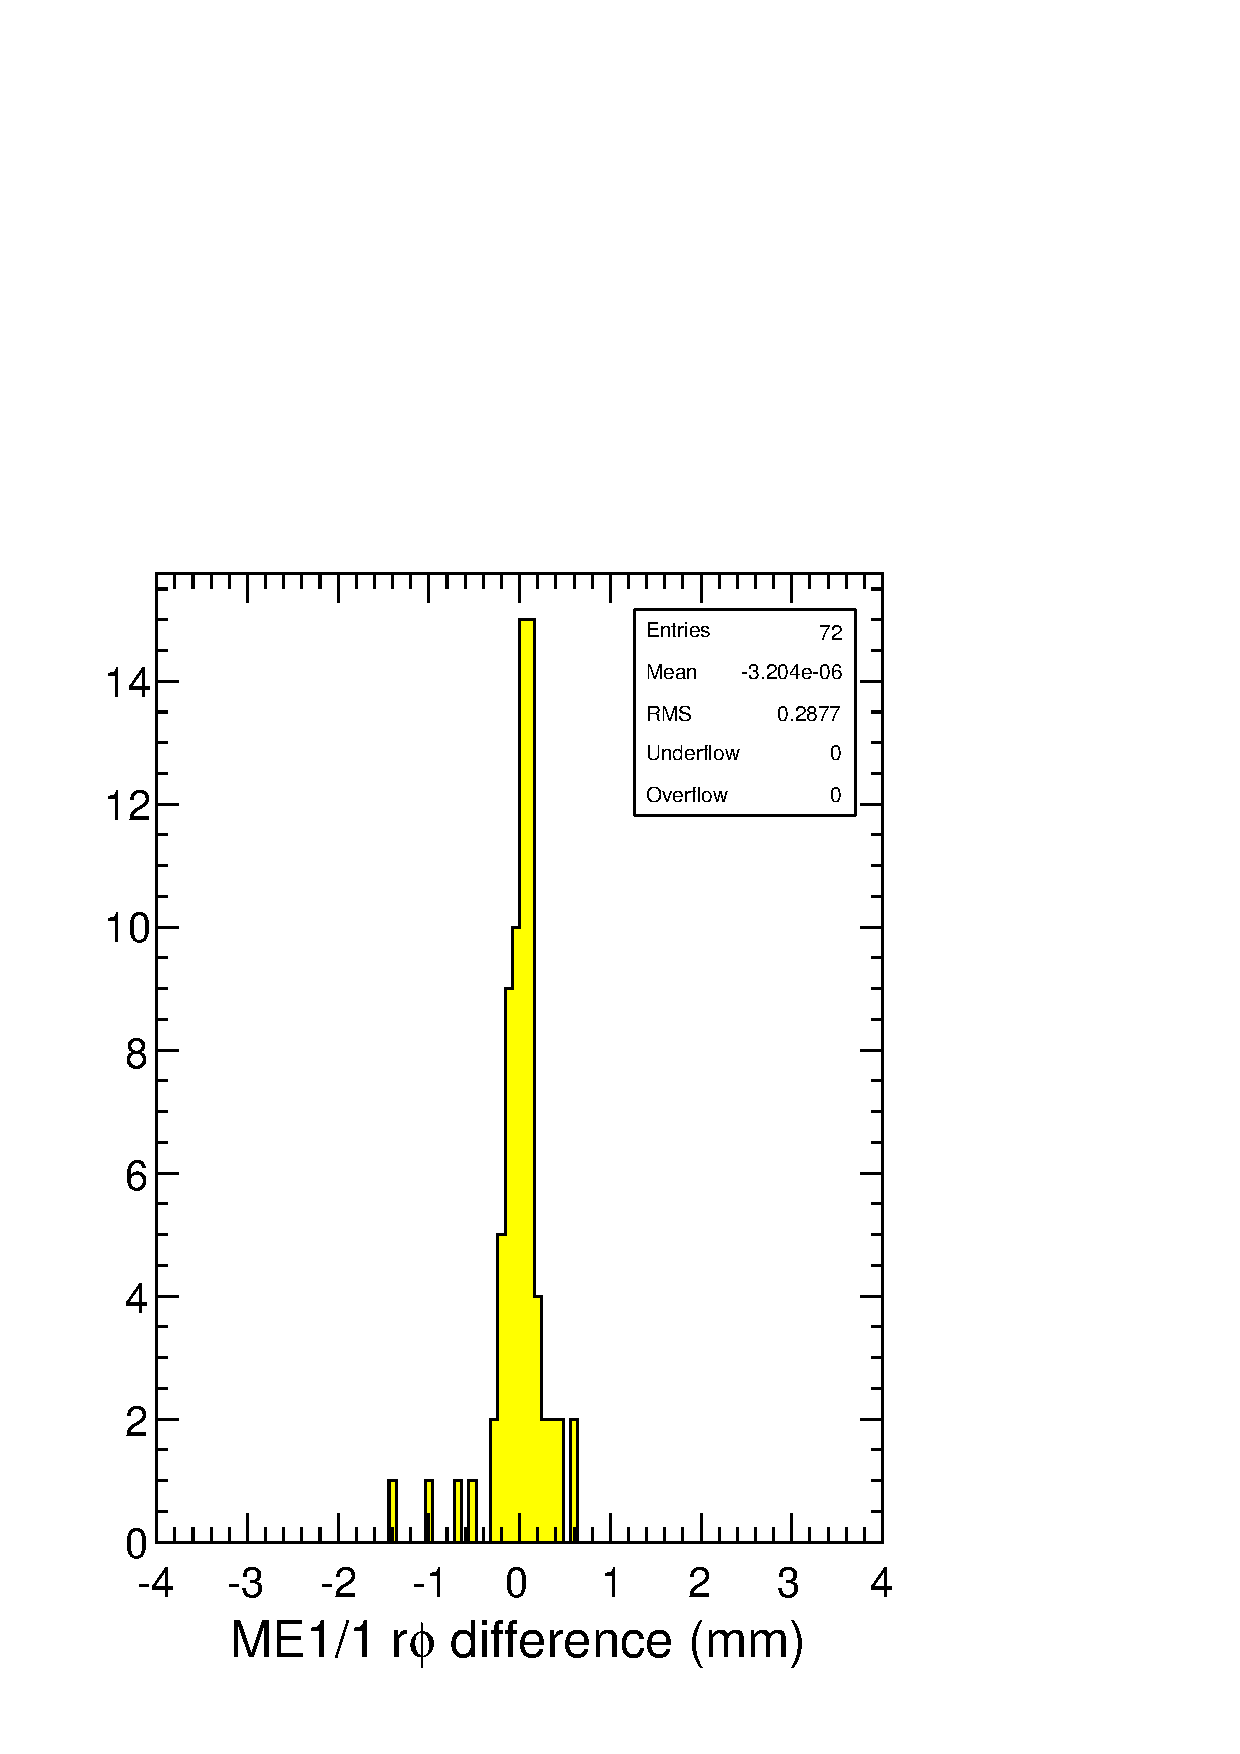
\includegraphics[width=0.32\linewidth]{noPhiYtoPhiY_me11.pdf}
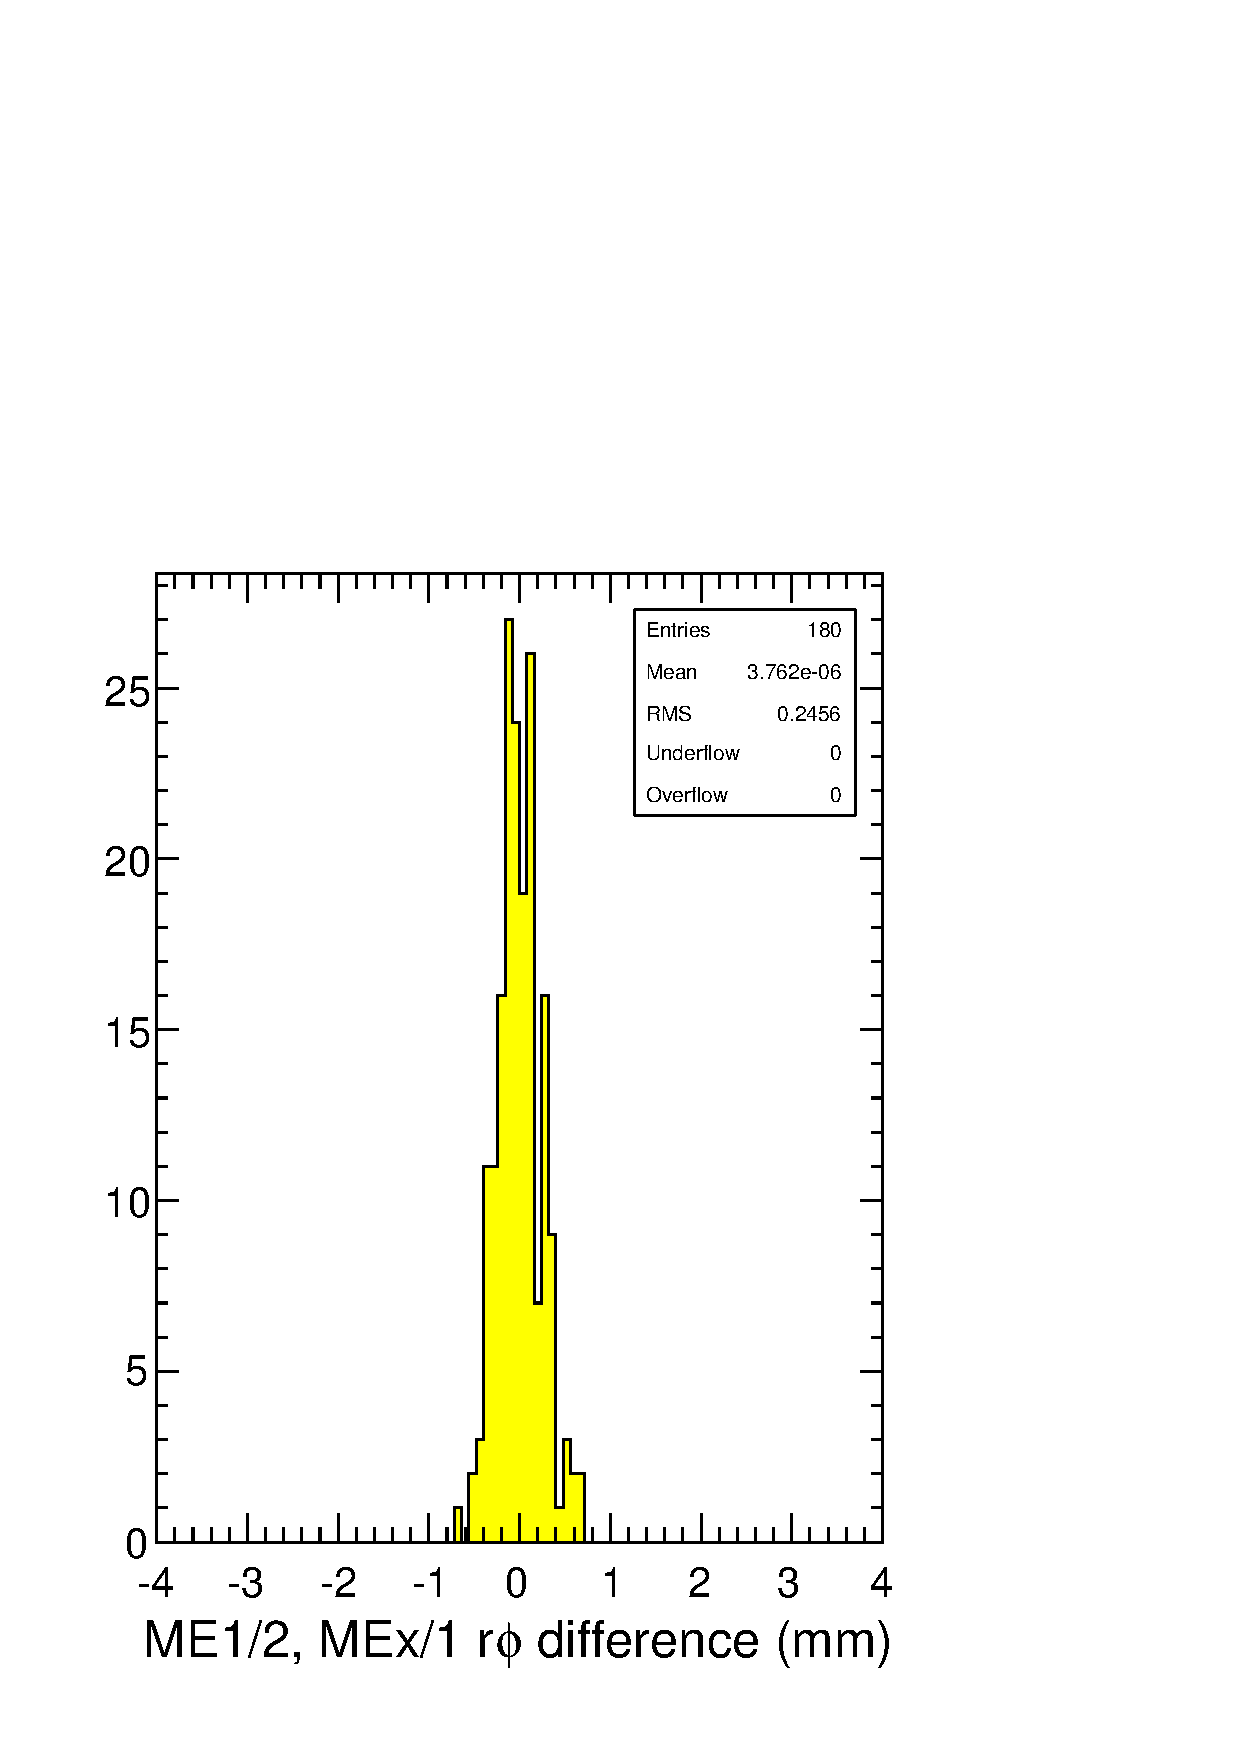
\includegraphics[width=0.32\linewidth]{noPhiYtoPhiY_inner.pdf}
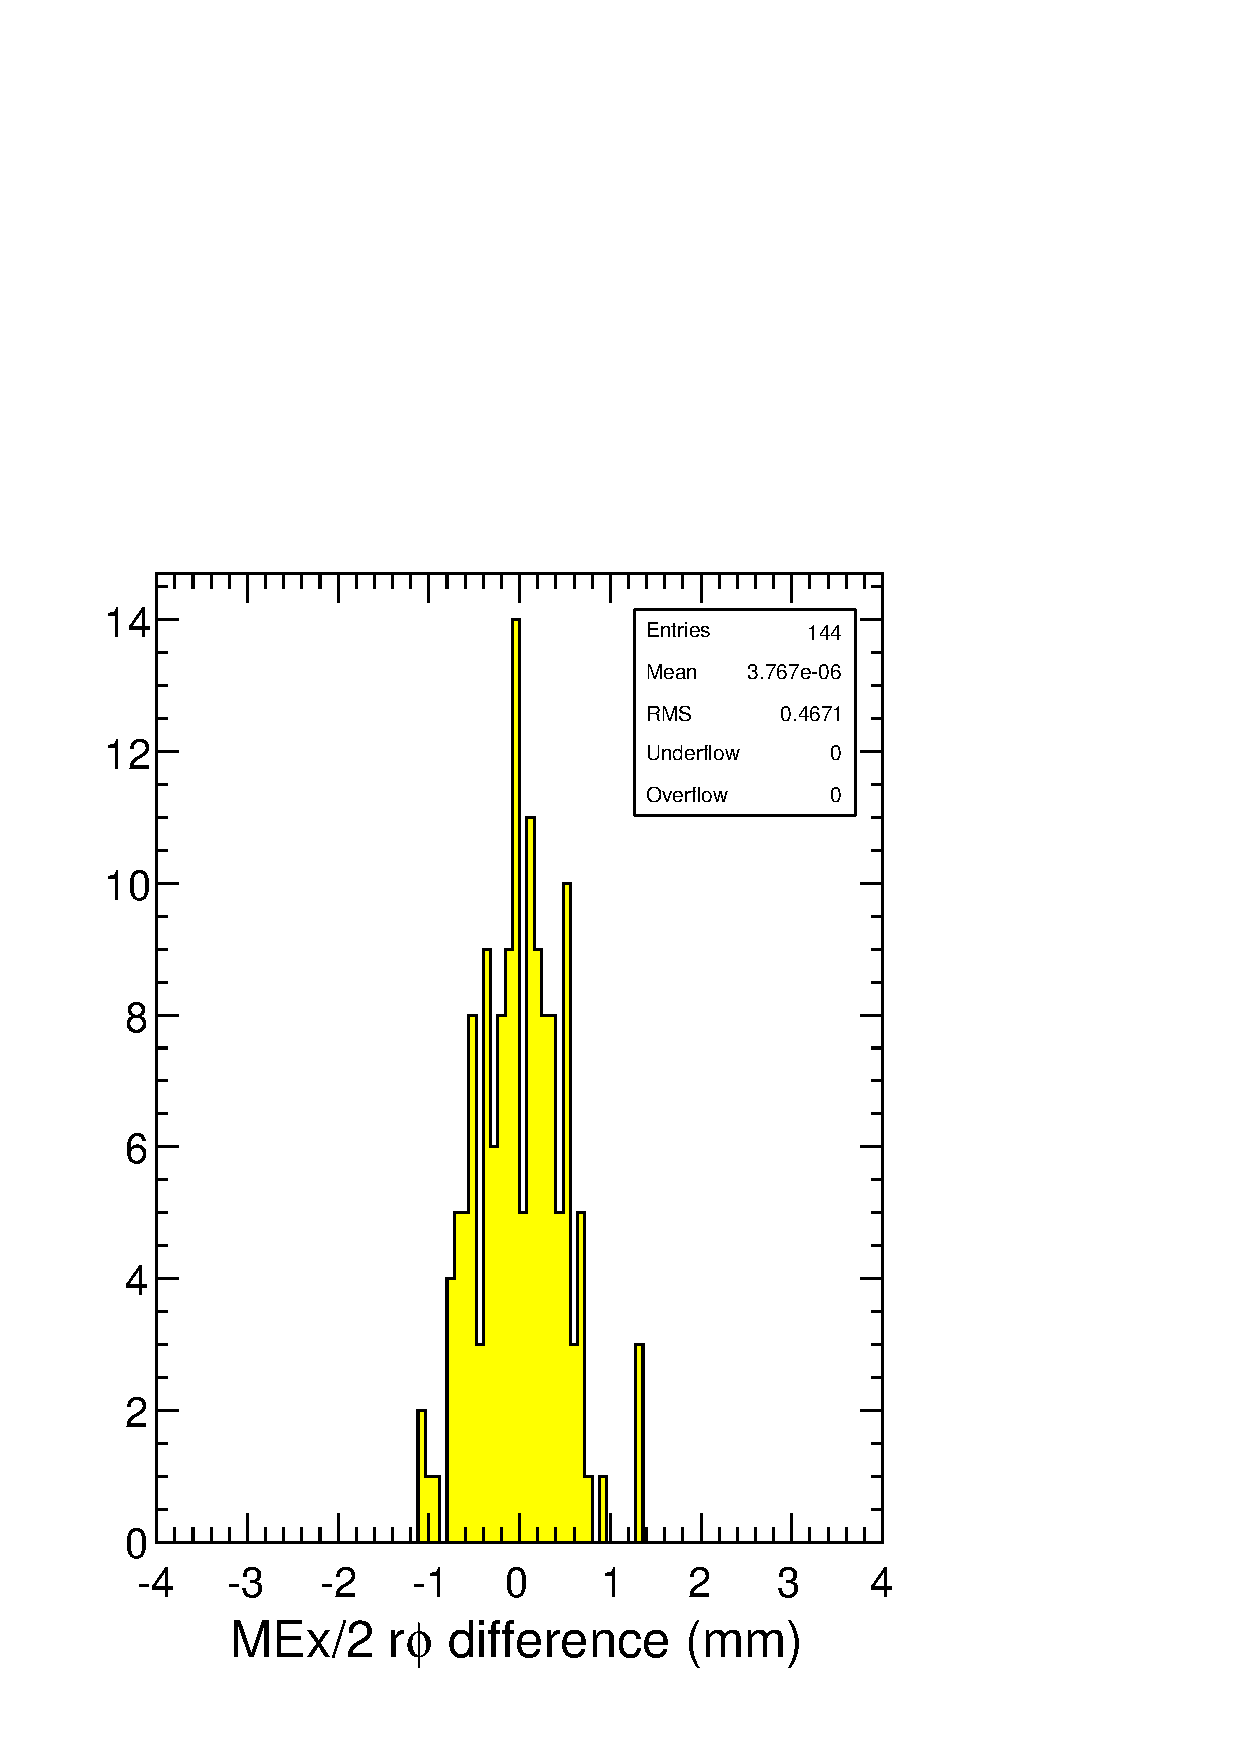
\includegraphics[width=0.32\linewidth]{noPhiYtoPhiY_outer.pdf}

\item 0.25--0.50~mm sensitivity
\end{itemize}
\end{frame}

\begin{frame}
\frametitle{Results: no PG $\to$ with PG}
\begin{itemize}

\item Photogrammetry constraint makes a big difference in outer rings:

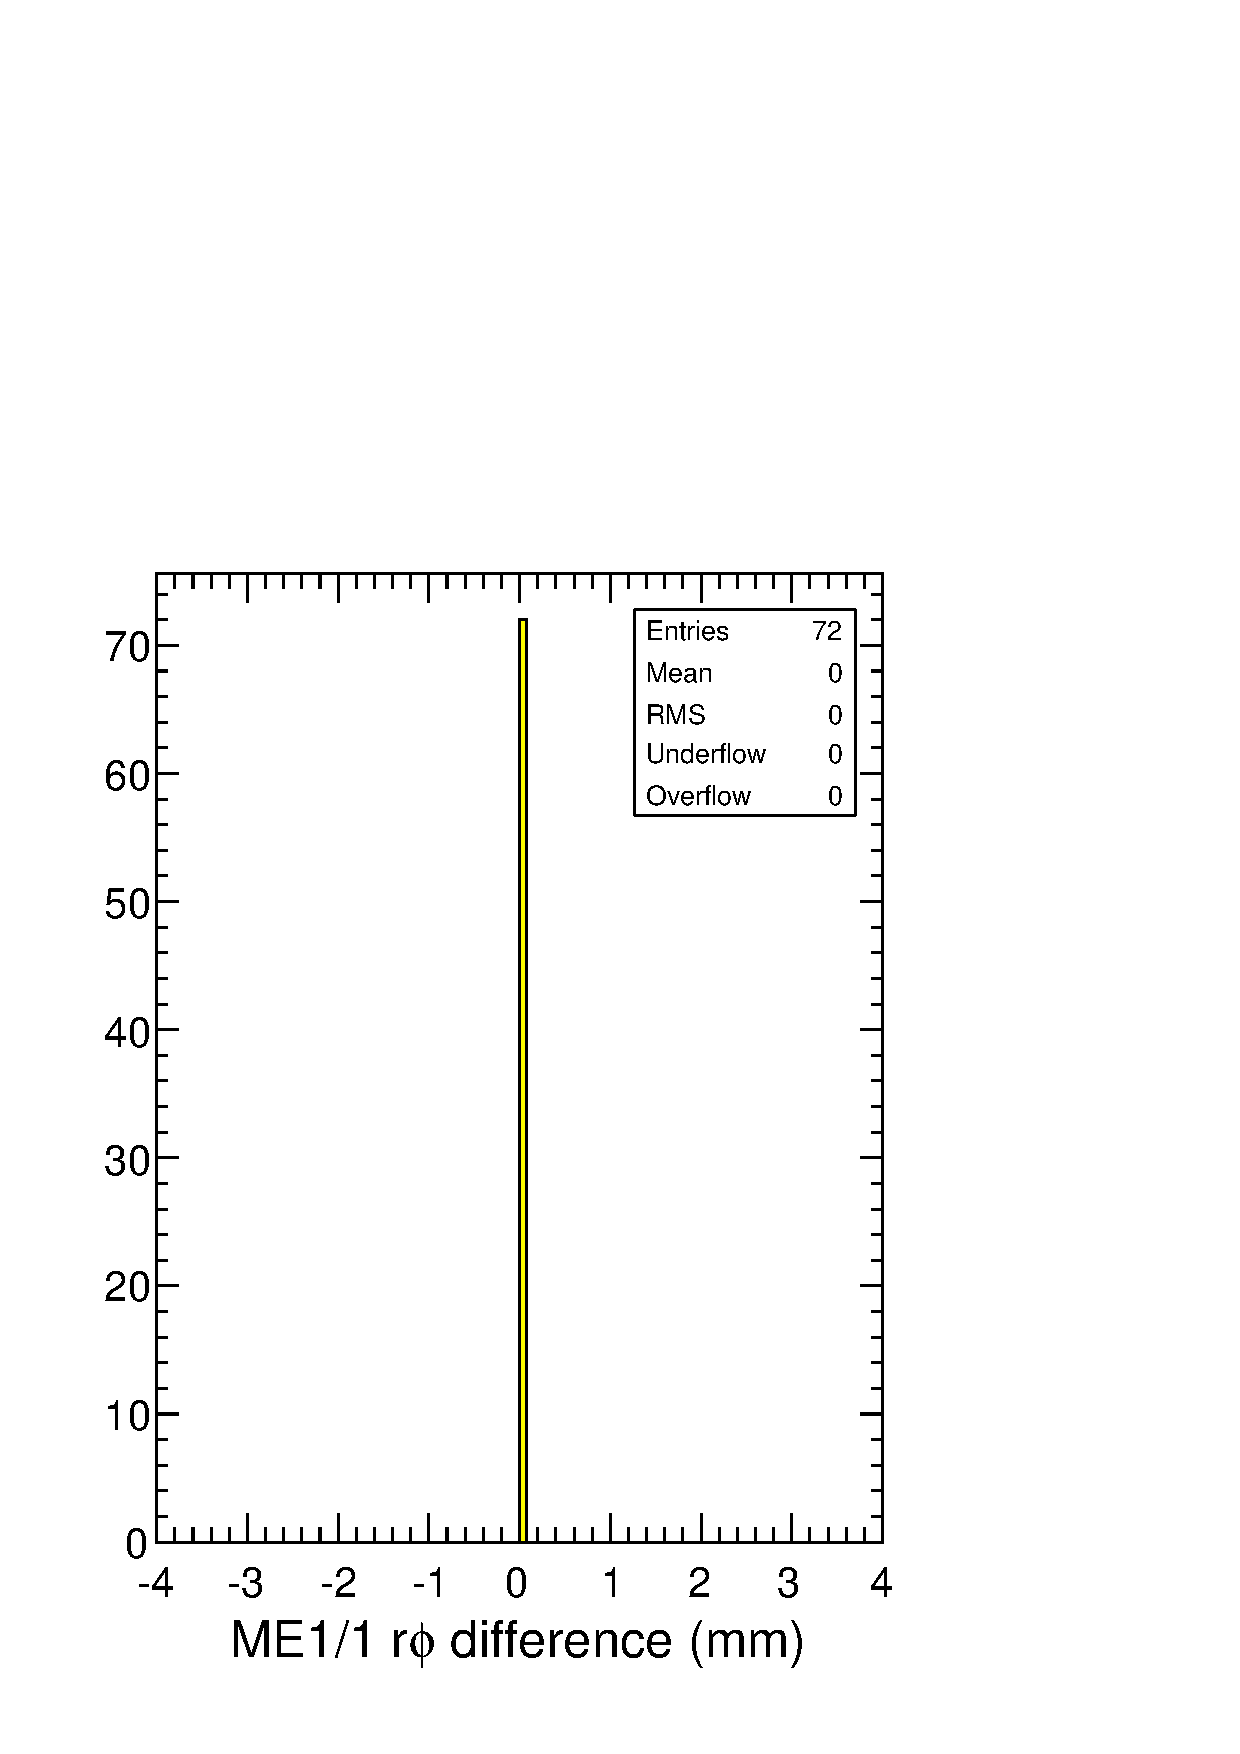
\includegraphics[width=0.25\linewidth]{withPGtoNoPG_me11.pdf}
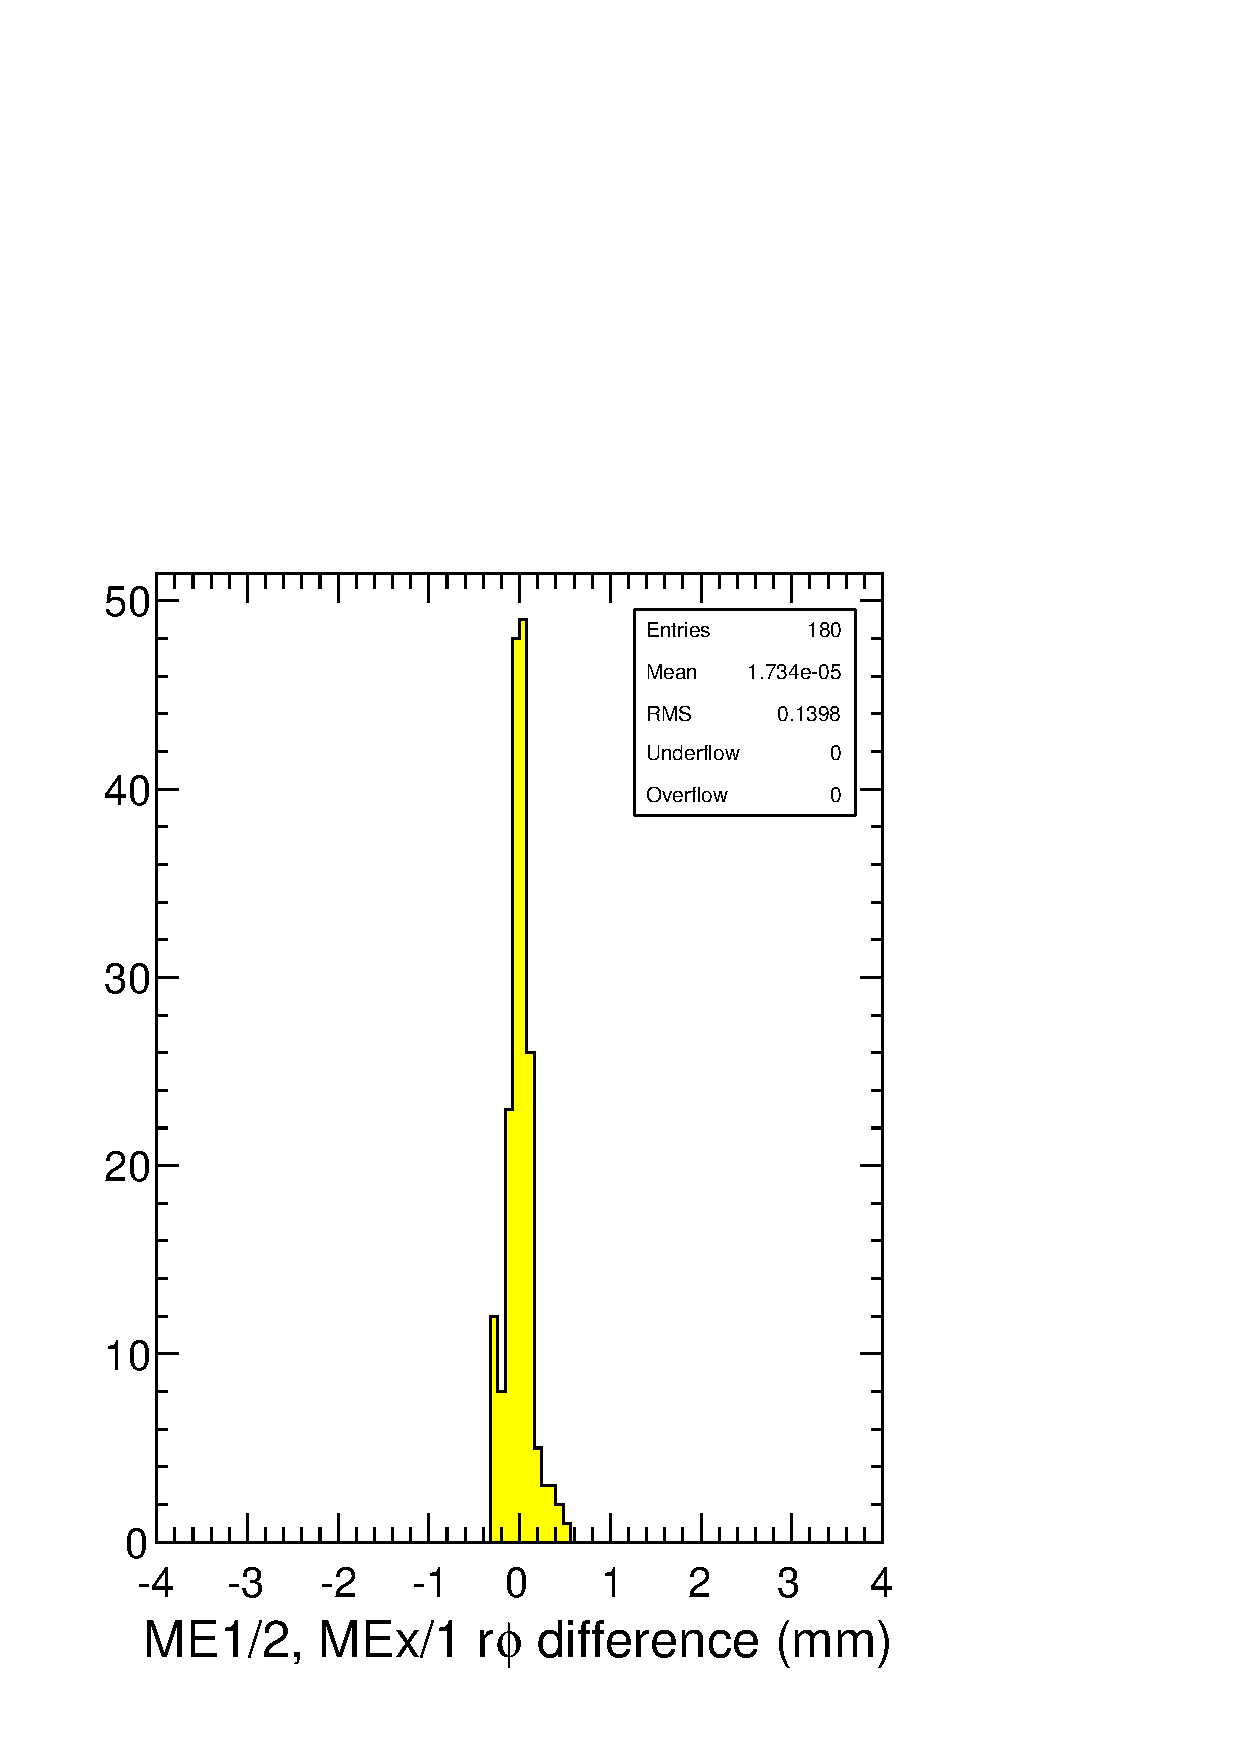
\includegraphics[width=0.25\linewidth]{withPGtoNoPG_inner.pdf}
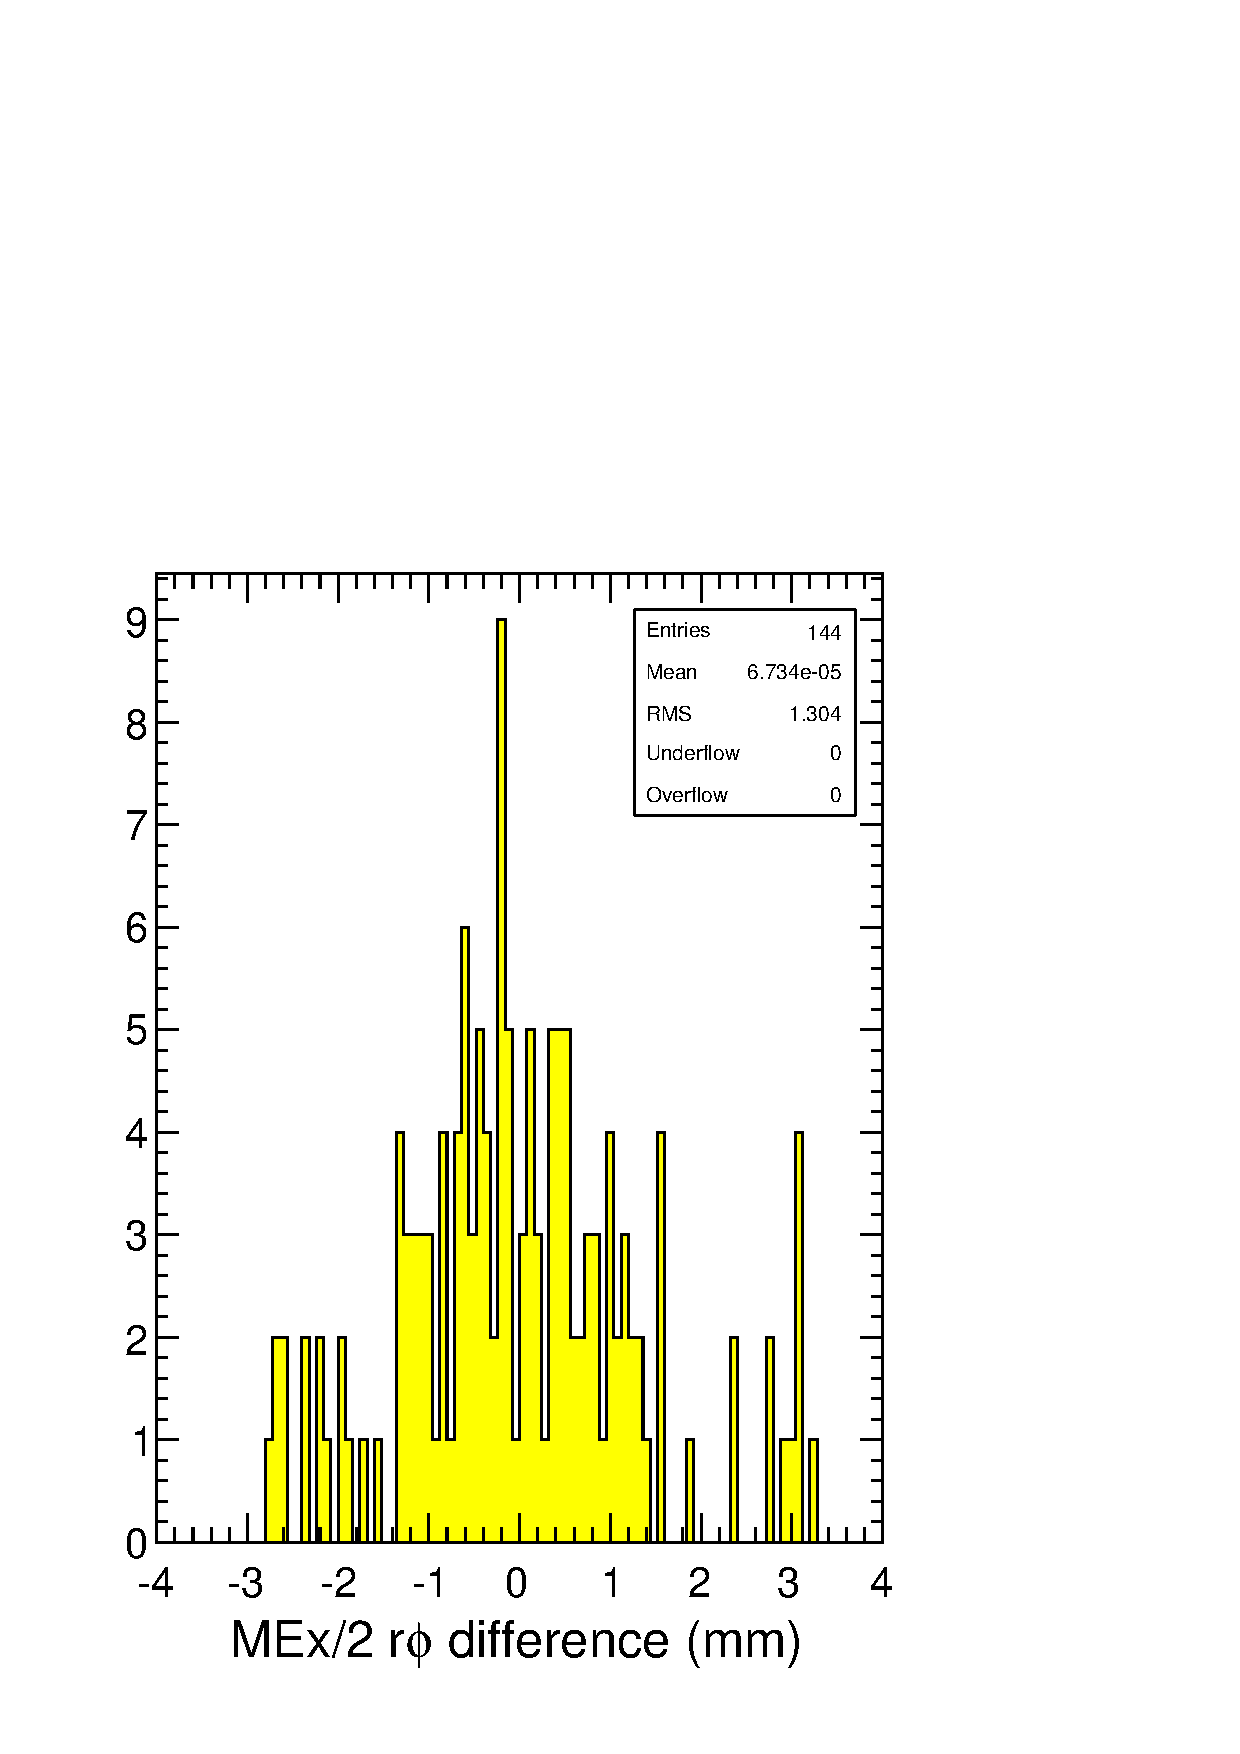
\includegraphics[width=0.25\linewidth]{withPGtoNoPG_outer.pdf}

\item ME$+$2/2: correction mainly at missing overlaps (good)
\item ME$+$3/2: systematic trend for all chambers (bad)

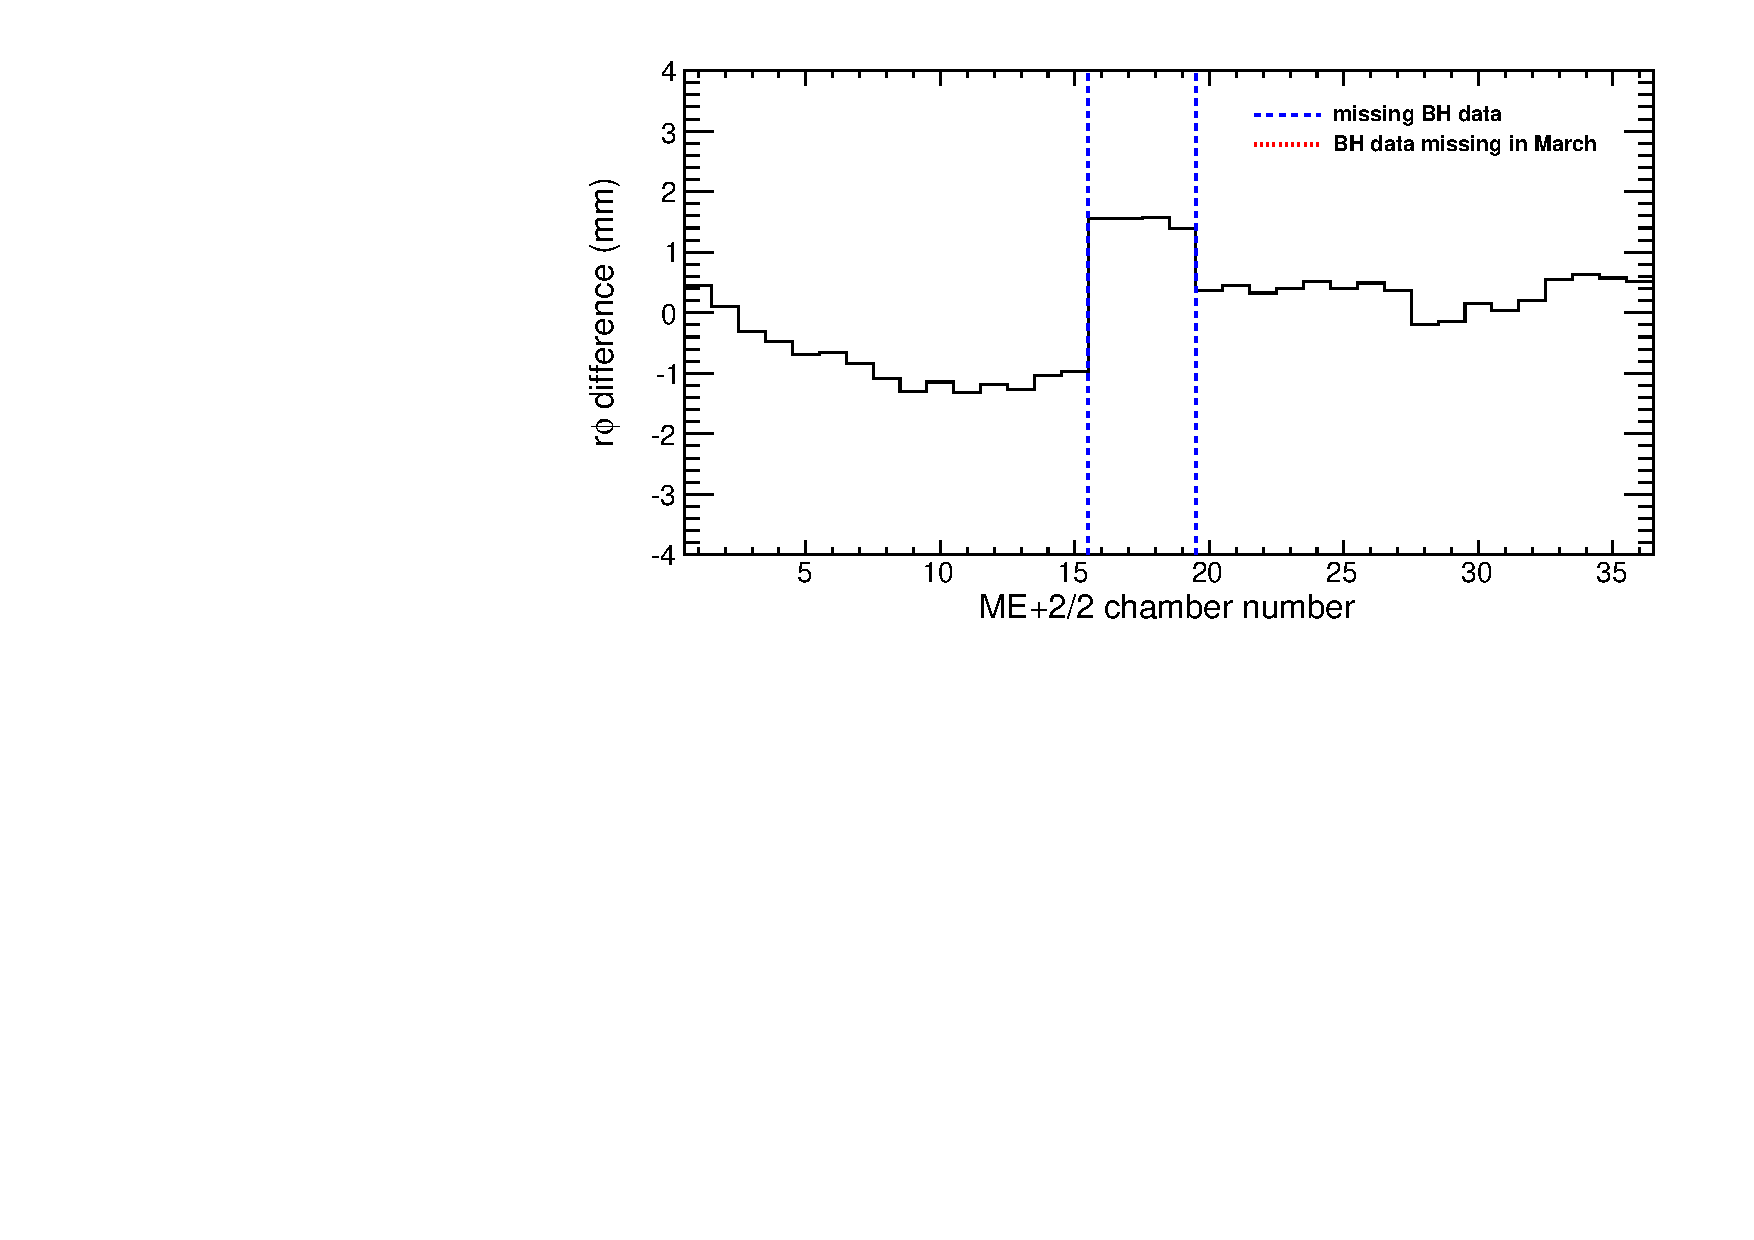
\includegraphics[width=0.5\linewidth]{withPGtoNoPG_mep22.pdf}
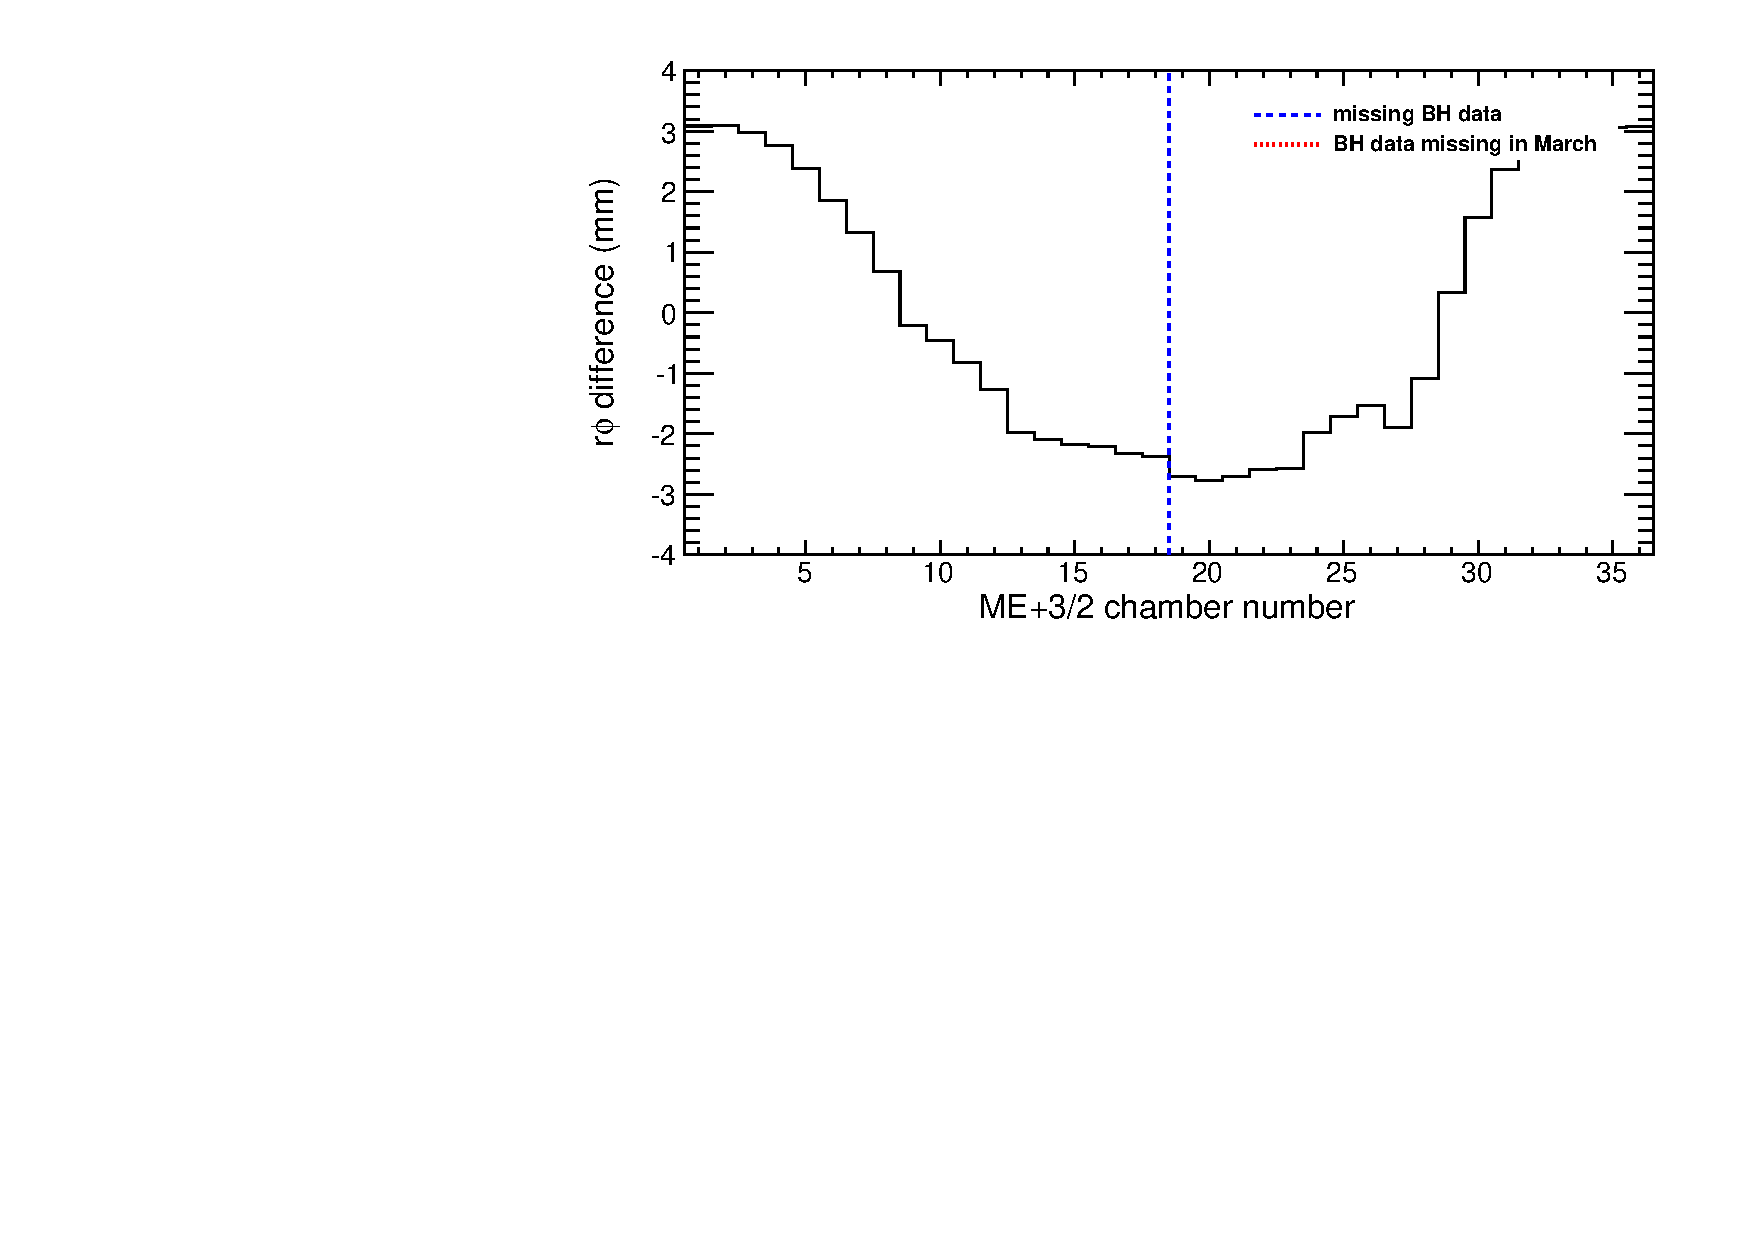
\includegraphics[width=0.5\linewidth]{withPGtoNoPG_mep32.pdf}

\end{itemize}
\end{frame}

\begin{frame}
\frametitle{Minimal use of PG}

\begin{itemize}
\item In the March alignment, the complete set of photogrammetry data
  was used with the beam-halo data in a combined fit (properly weighted)
\item This forces the aligned result to be centered on the
  photogrammetry's $x$-$y$ origin (differences appear as sinusoidal
  deviations in $r\phi$ vs.\ $\phi$ curves, most dramatically in ME$+$3/2)
\item This is especially undesirable after the rings have been aligned
  with respect to the tracker
\item Solution: minimize use of constraints
\begin{itemize}
\item only ``patch holes'' in beam-halo data with photogrammetry
\item only one photogrammetry constraint allowed per ring (this is possible with the current pattern of holes)
\item allow PGFrame to float as a free parameter in the alignment fit
\end{itemize}
\end{itemize}
\end{frame}

\begin{frame}
\frametitle{Minimal use of PG}

\begin{itemize}
\item Complete set of constraints on finalized beam-halo alignment

{\scriptsize
\begin{tabular}{r l}
Photogrammetry & ME$+$4/1/14 and ME$+$4/1/15 \\
constraints & ME$+$3/2/18 and ME$+$3/2/19 \\
& ME$+$2/2/19 and ME$+$2/2/20 \\
& ME$+$2/1/01 and ME$+$2/1/02 \\
& ME$+$1/2/14, ME$+$1/2/15, and ME$+$1/2/16 \\
& ME$-$1/2/33 and ME$-$1/2/34 \\
& ME$-$2/1/06 and ME$-$2/1/07 \\
& ME$-$2/2/02, ME$-$2/2/03, and ME$-$2/2/04
\end{tabular}}

\item Also adding measurements from TrackerMuons used to ``patch
  holes'' in ME1/1 data (in lieu of photogrammetry)

{\scriptsize
\begin{tabular}{r l}
Constraints from & ME$+$1/1/01 and ME$+$1/1/03 \\
TrackerMuon residuals & ME$+$1/1/19 and ME$+$1/1/21 \\
& ME$+$1/1/30 and ME$+$1/1/31 \\
& ME$-$1/1/14 and ME$-$1/1/16 \\
& ME$-$1/1/33 and ME$-$1/1/35 \\
& ME$-$1/1/30 and ME$-$1/1/31 \\
\end{tabular}}

\end{itemize}
\end{frame}

\begin{frame}
\frametitle{Results: no PG $\to$ minimal PG}
\begin{center}
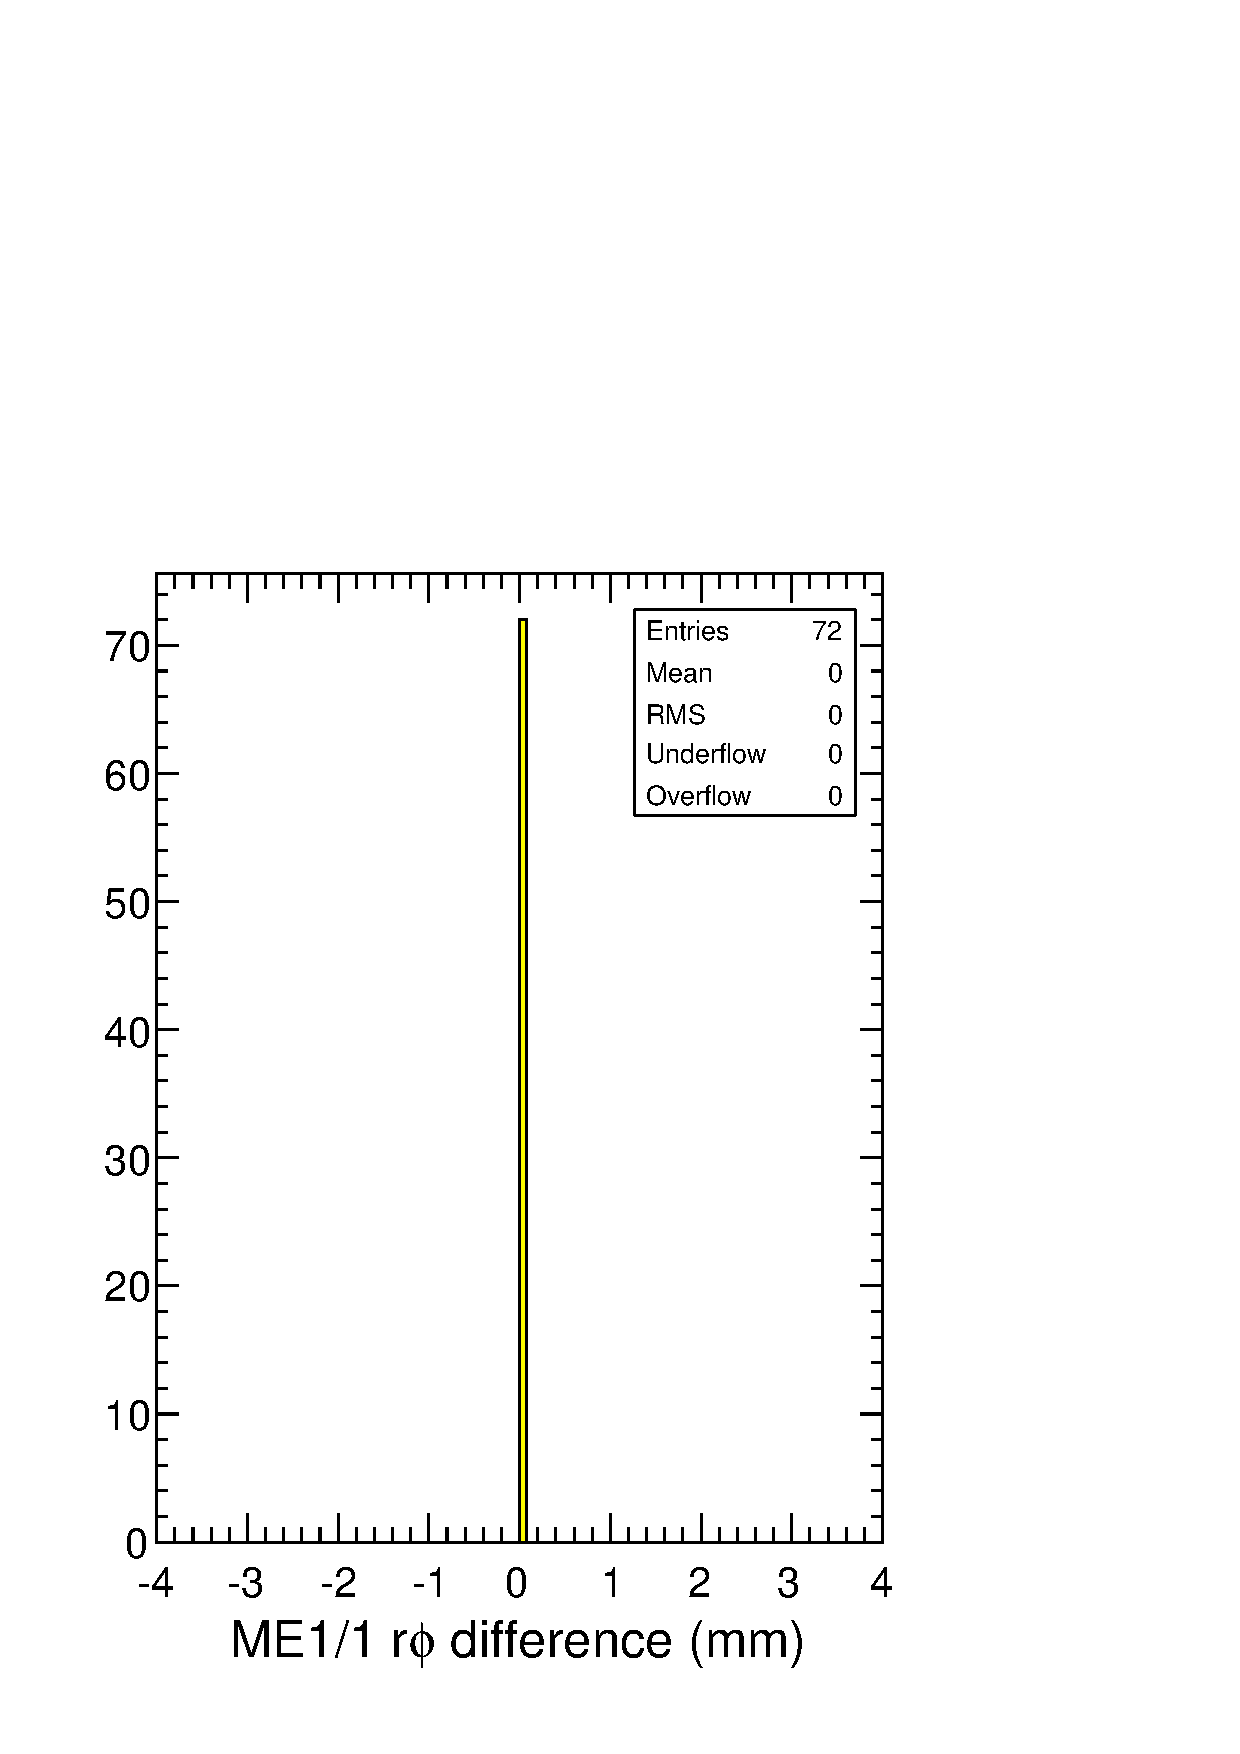
\includegraphics[width=0.27\linewidth]{effectofholes_me11.pdf}
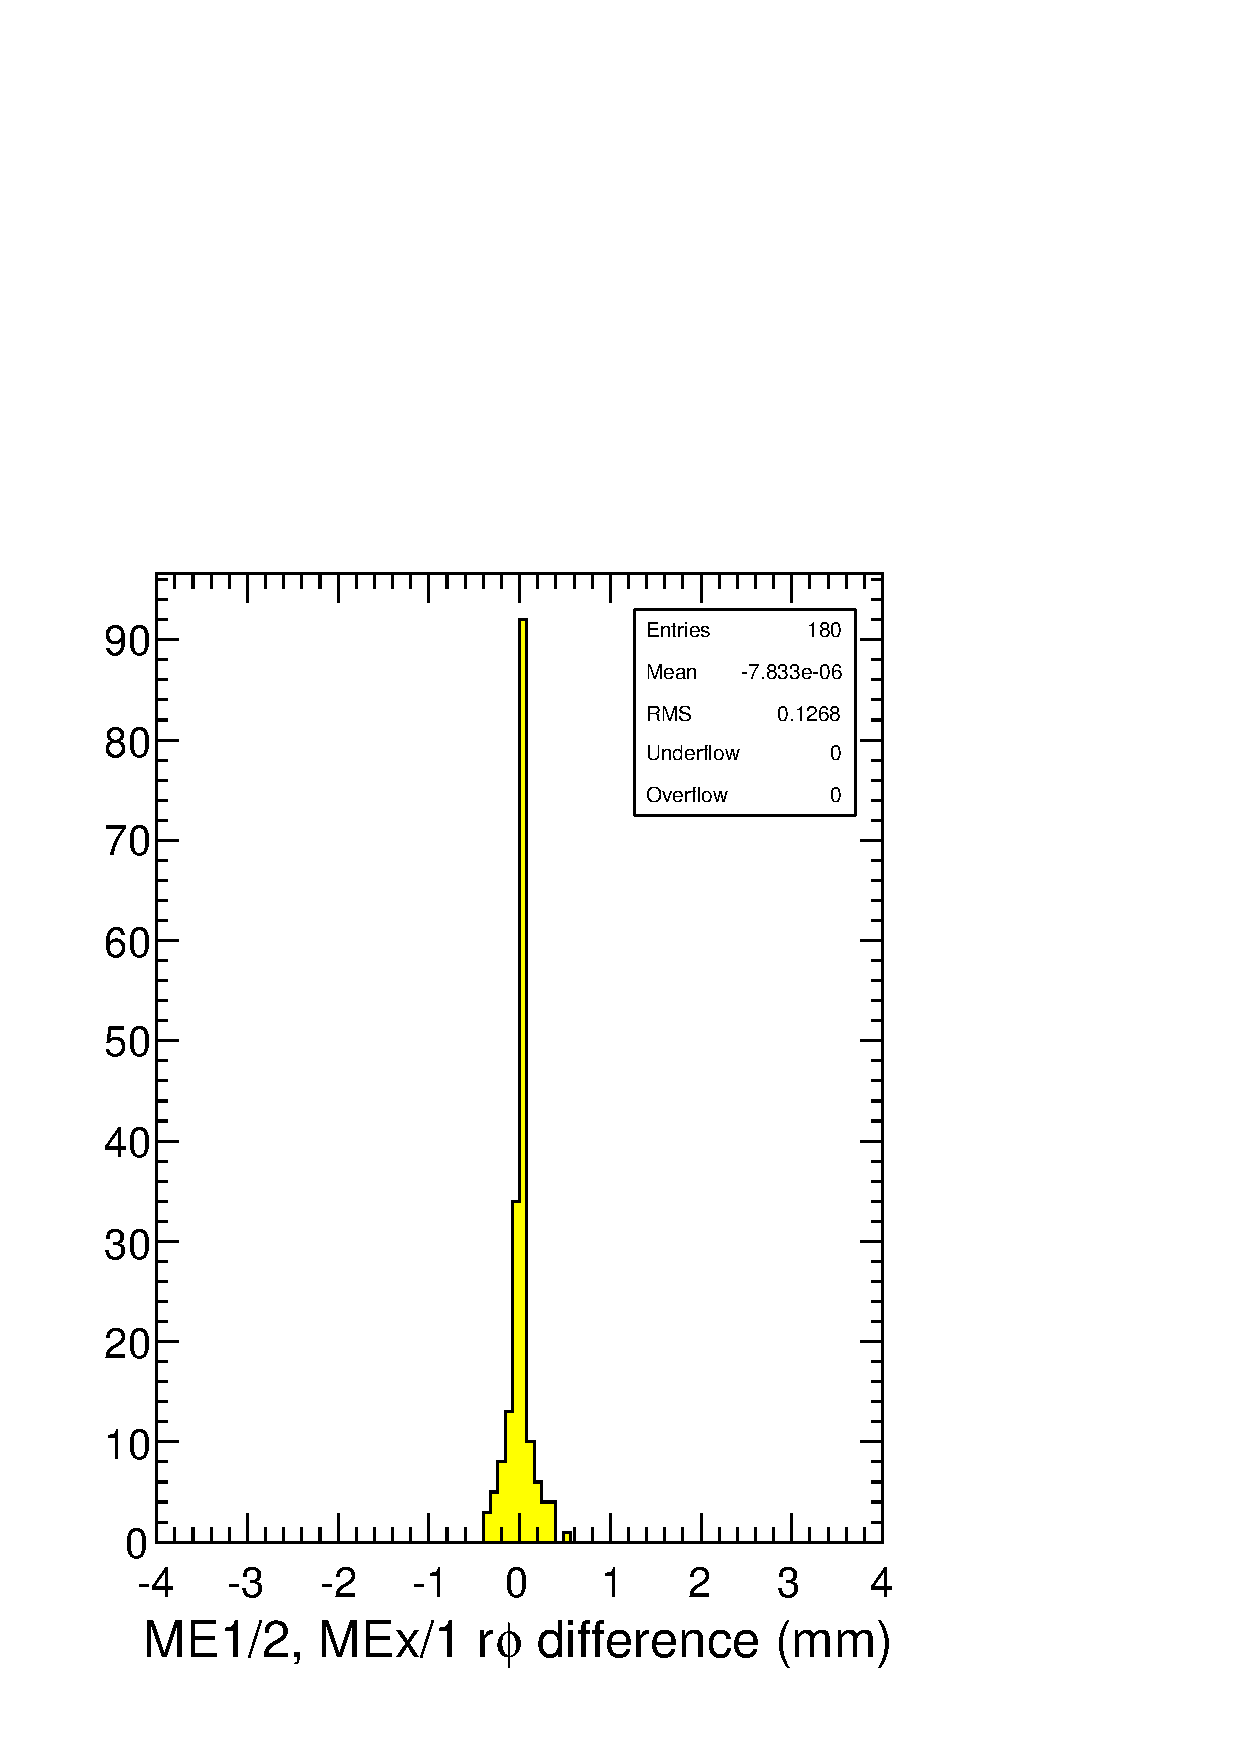
\includegraphics[width=0.27\linewidth]{effectofholes_inner.pdf}
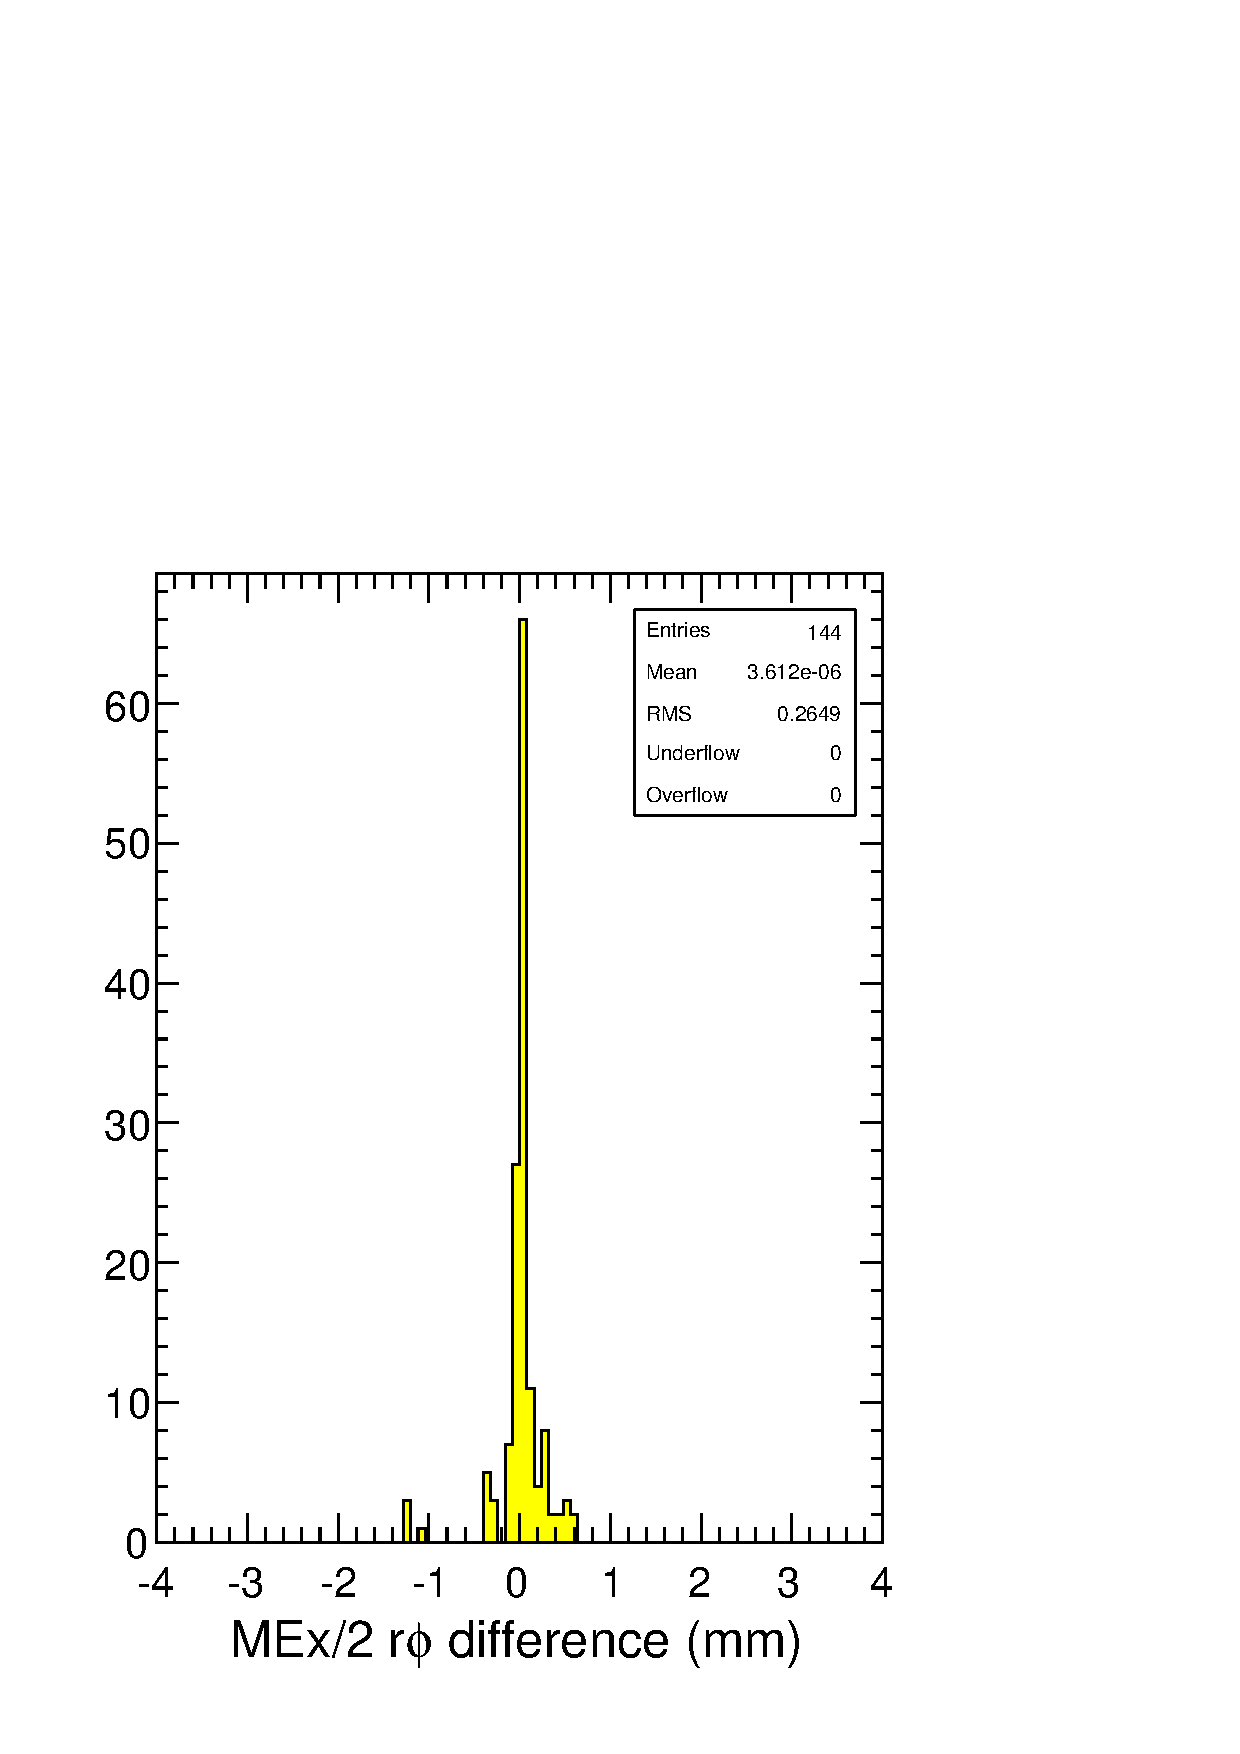
\includegraphics[width=0.27\linewidth]{effectofholes_outer.pdf}
\end{center}

\vspace{-0.4 cm}
\begin{itemize}
\item ME$+$2/2: still corrects the parts of the ring with missing data
\item ME$+$3/2: no longer pulls the whole ring to a new center

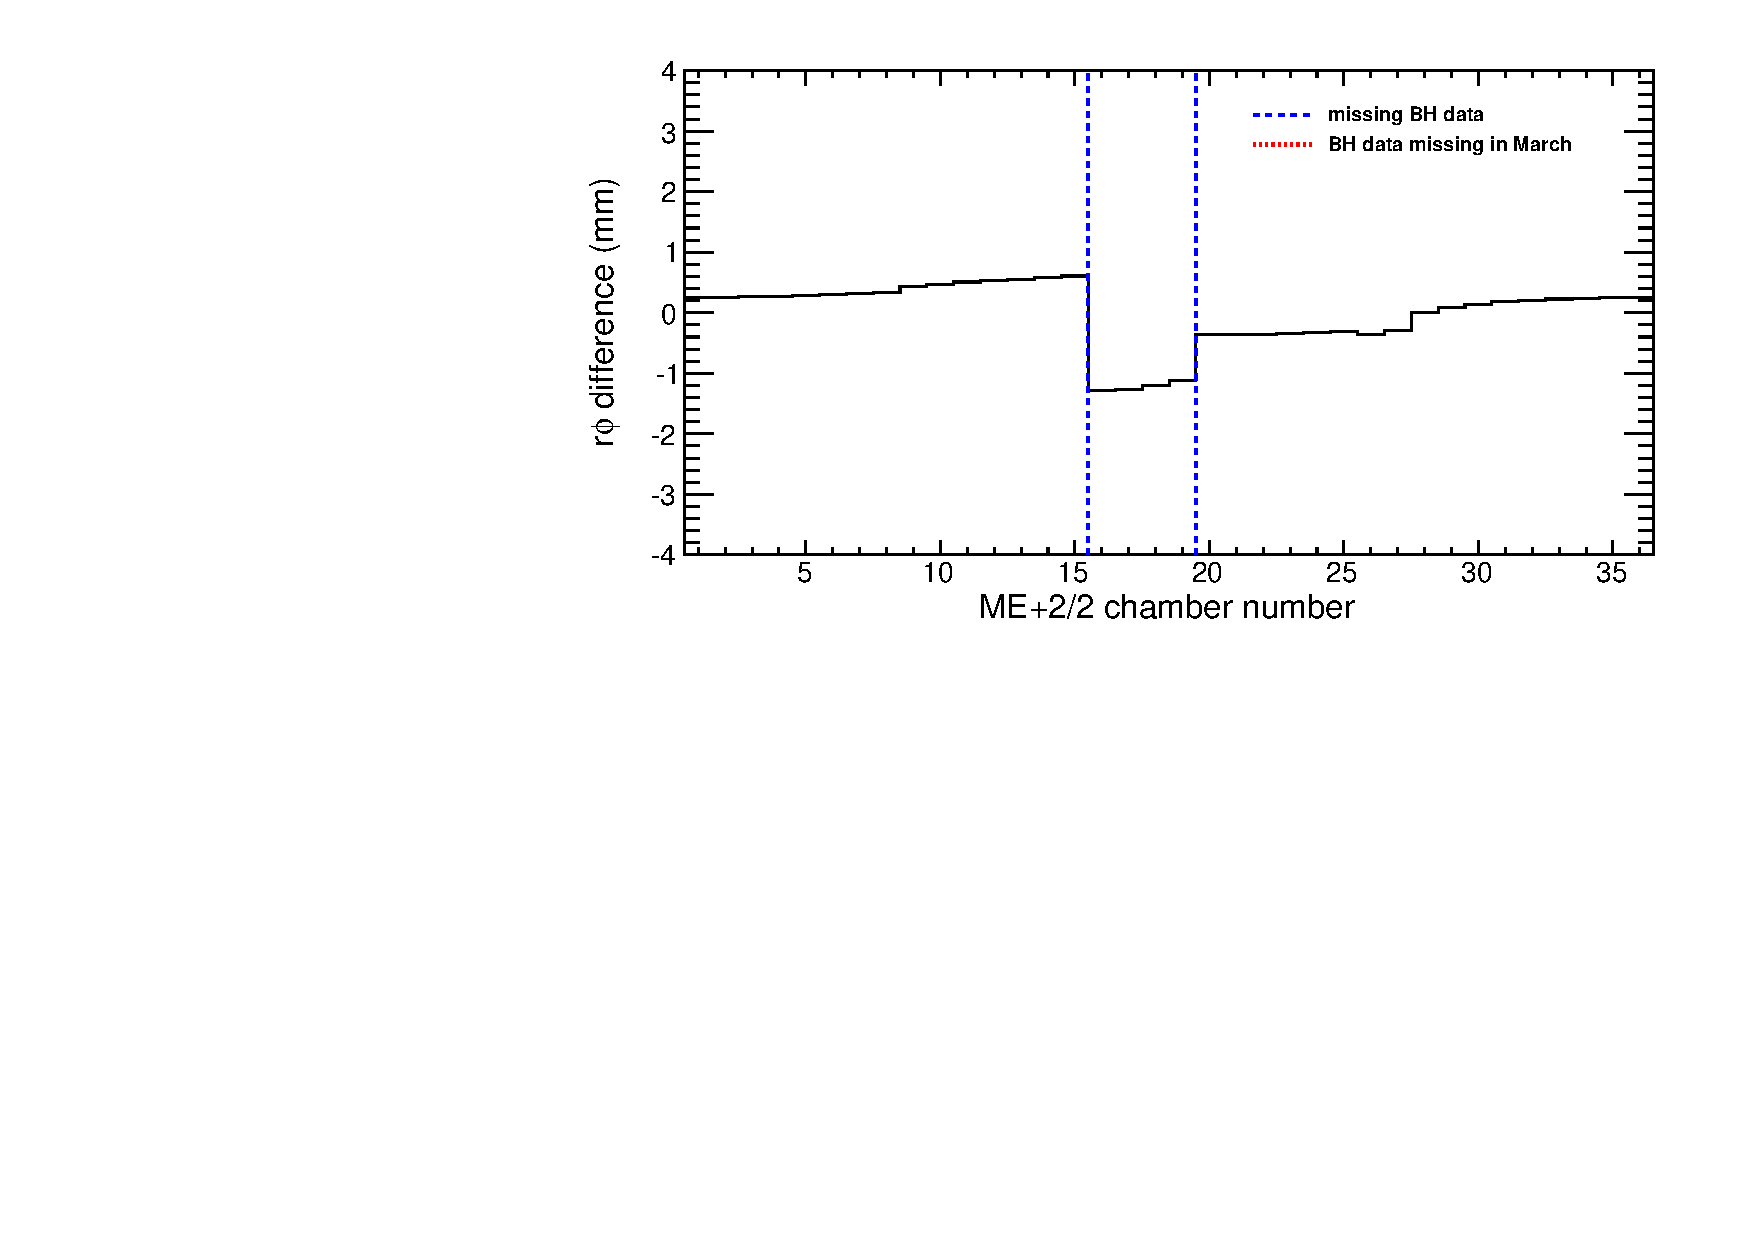
\includegraphics[width=0.5\linewidth]{effectofholes_mep22.pdf}
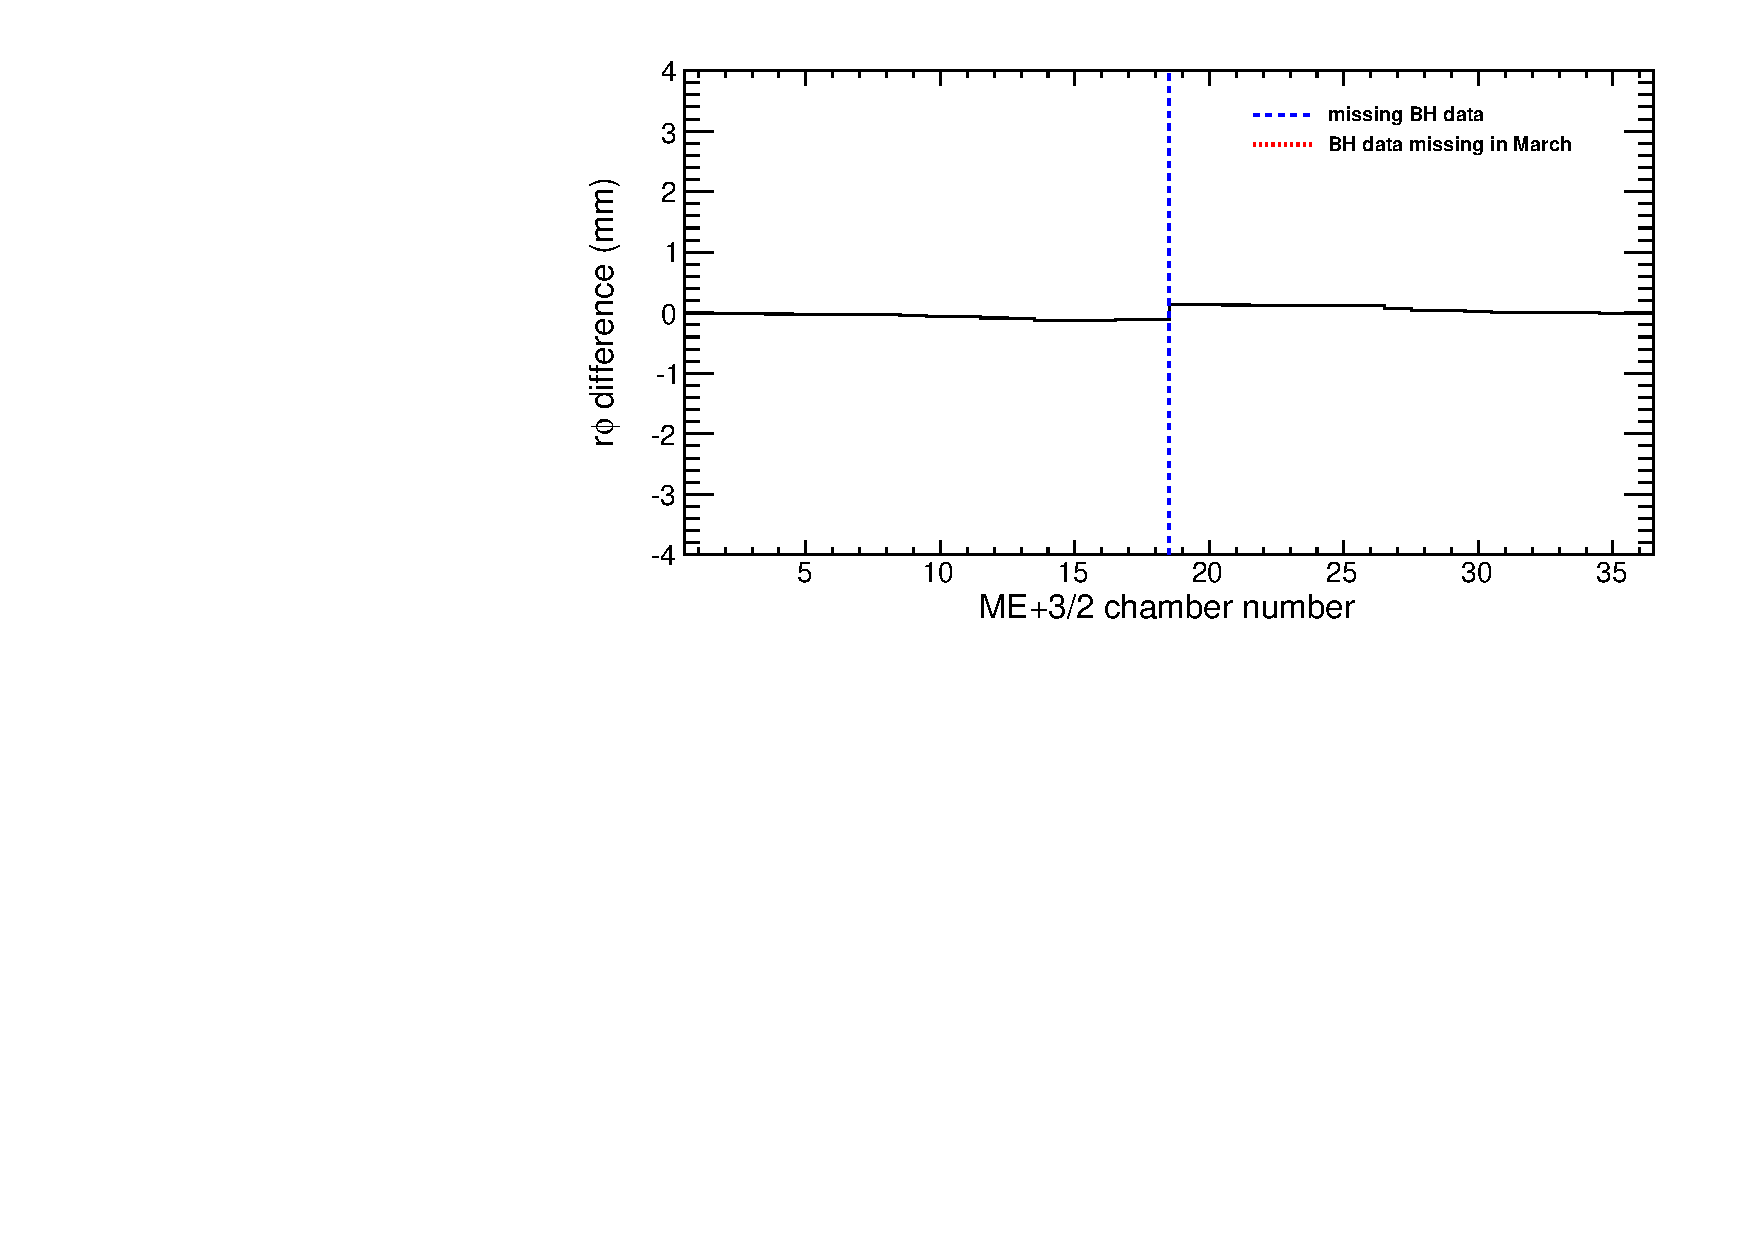
\includegraphics[width=0.5\linewidth]{effectofholes_mep32.pdf}

\end{itemize}
\end{frame}

\begin{frame}
\frametitle{Unconstrained modes of the fit}

\begin{itemize}
\item By definition, the fit is insensitive to global shifts:
\begin{center}
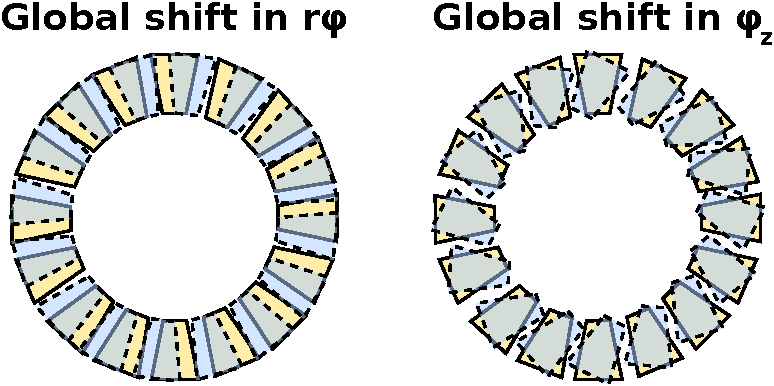
\includegraphics[width=0.7\linewidth]{global_shifts.pdf}
\end{center}

\item Global shifts are not introduced by the algorithm: the value of
  these unmeasured degrees of freedom are set to zero

\item The $r\phi$ global shifts are later corrected by the whole-ring
  position measurement relative to the tracker, so they are resolved
  in the final geometry

\item Any global shifts in $\phi_z$ are not
\end{itemize}
\end{frame}

\begin{frame}
\frametitle{Unconstrained modes of the fit}

\hfill 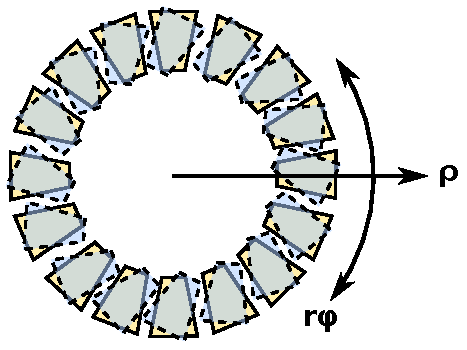
\includegraphics[width=0.35\linewidth]{global_shifts2.pdf}

\vspace{-2.7 cm}
\begin{itemize}
\item My observation at the end of the new \\ constants preparation:

\item I think we may be seeing evidence for \\ coherent $\phi_z$ torsion
  in the TrackerMuon \\ residuals (Vadim's plots)

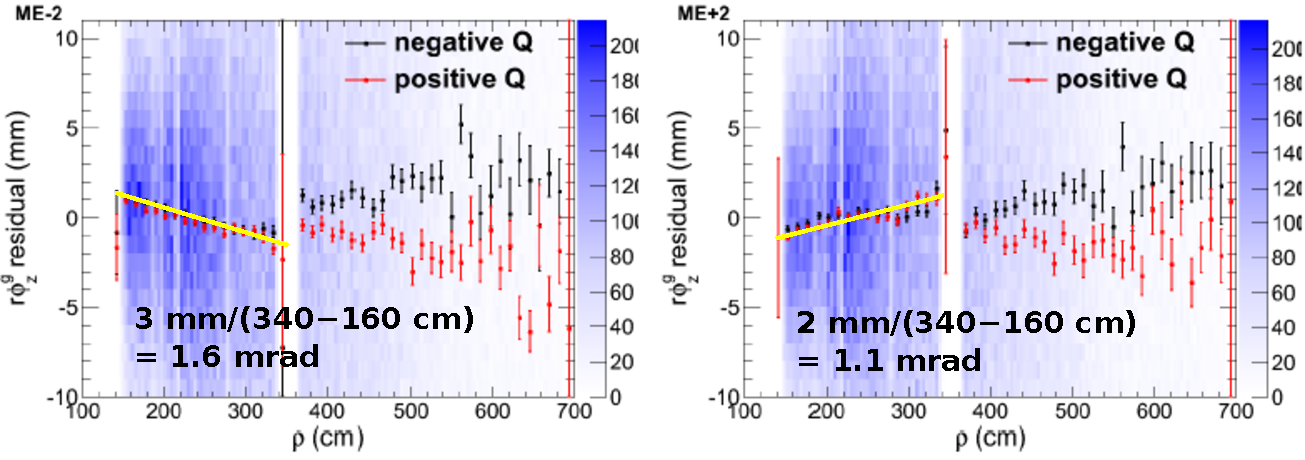
\includegraphics[width=\linewidth]{rphi_plots_vs_rho.pdf}

\item Treated as a systematic error in the ring-alignment procedure

\item This is the next level of detail, to be corrected in the next
  round; \\ if the Reference-Target algorithm is applied to collisions,
  it would be resolved directly
\end{itemize}
\end{frame}

%% \begin{frame}
%% \frametitle{Outline}
%% \begin{itemize}\setlength{\itemsep}{0.75 cm}
%% \item 
%% \end{itemize}
%% %% \hspace{-0.83 cm} \textcolor{darkblue}{\Large Outline2}
%% \end{frame}

%% \section*{First section}
%% \begin{frame}
%% \begin{center}
%% \Huge \textcolor{blue}{First section}
%% \end{center}
%% \end{frame}

\begin{frame}
\frametitle{Conclusions}
\begin{itemize}
\item Internal ring alignment has been updated with beam-halo muons
\begin{itemize}
\item using the $10\times$ larger beam-halo dataset we collected
  during collisions (before the halo-trigger was retired
  Sep.~1)
\item improved $\phi_y$ measurement with collisions before applying
  beam-halo alignment procedure: good agreement with historical
  results but negligible impact on beam-halo alignment
\item minimized global-position bias from photogrammetry by only using
  it to ``fill holes'' in the overlaps data
\item new geometry is presented for approval
\end{itemize}

\item The next step (beyond this sign-off) is to apply the
  Reference-Target procedure with collisions muons
\begin{itemize}
\item Reference-Target is much more direct but relies on long propagations of tracker-tracks
\item obtaining the same result would be a non-trivial validation
\item but we should keep in mind which degrees of freedom the
  beam-halo does not constrain when we do that comparision
\end{itemize}

\end{itemize}
\label{numpages}
\end{frame}

\end{document}
